\documentclass{article}

\usepackage{iclr2027_conference}
\usepackage{iftex}
\ifPDFTeX
  \usepackage{times}
\else
  \usepackage{fontspec}
  \setmainfont{STIX Two Text}
  \setsansfont{Liberation Sans}[Scale=MatchLowercase]
  \setmonofont{Liberation Mono}[Scale=MatchLowercase]
\fi
\usepackage{amsmath,amssymb,mathtools,bm}
\usepackage{booktabs,multirow,array,tabularx,longtable}
\usepackage{xcolor}
\usepackage{colortbl}
\usepackage{arydshln}
\ADLinactivate
\usepackage{graphicx}
\usepackage{float}
\usepackage{placeins}
\usepackage{microtype}
\usepackage{tikz}
\usetikzlibrary{arrows.meta,backgrounds,calc,fit,positioning,shapes.geometric}
\usepackage{hyperref}
\usepackage{url}
\hypersetup{hidelinks}

\setlength{\textfloatsep}{6pt plus 2pt minus 2pt}
\setlength{\floatsep}{6pt plus 2pt minus 2pt}
\setlength{\intextsep}{6pt plus 2pt minus 2pt}
\setlength{\abovecaptionskip}{3pt}
\setlength{\belowcaptionskip}{0pt}
\makeatletter
\renewcommand{\fnum@figure}{\textbf{\figurename~\thefigure}}
\renewcommand{\fnum@table}{\textbf{\tablename~\thetable}}
\setlength{\@fptop}{0pt}
\setlength{\@fpsep}{10pt plus 2pt minus 2pt}
\setlength{\@fpbot}{0pt plus 1fil}
\makeatother

\definecolor{flowblue}{HTML}{2F65A7}
\definecolor{flowteal}{HTML}{2A9D8F}
\definecolor{floworange}{HTML}{E07A35}
\definecolor{flowred}{HTML}{B42318}
\definecolor{flowgray}{HTML}{667085}
\definecolor{flowlight}{HTML}{F2F4F7}

\newcommand{\method}{ZoomST}
\newcommand{\asnll}{\textsf{All-Source NLL}}
\newcommand{\Rset}{\mathcal{R}}
\newcommand{\Pset}{\mathcal{P}}
\newcommand{\support}{\mathcal{S}}
\newcommand{\stopgrad}{\operatorname{sg}}
\newcommand{\diag}{\operatorname{diag}}

\title{ZoomST: Pretraining Spatial Transcriptomic\\Representations with Learnable\\Cross-Granularity Transformations}

\author{Anonymous authors}


\begin{document}

\maketitle

\begin{abstract}
Tissue function depends on spatial organization across scales, from cellular neighborhoods to anatomical regions. Expanding spatial context around a focal location yields related but distinct representations of tissue organization at different granularities. Although existing spatial transcriptomics pretraining models incorporate multiscale context for representation learning, they do not explicitly learn how representations change as spatial context expands. We introduce ZoomST, a self-supervised framework that jointly learns granularity-specific, cross-scale-compatible representations and transformations among them. ZoomST combines molecular-spatial dual-view alignment within each granularity with a soft distributional equivariance constraint across granularities. Across held-out mouse sections spanning all sampled developmental stages, frozen ZoomST representations outperform the evaluated pretrained baselines and remain competitive with target-fitted methods for tissue mapping. Anatomical analysis in a mouse developmental atlas further illustrates the complementary information captured by fine and coarse spatial context. Continuous transformations learned only from discrete training granularities predict representations at unseen intermediate spatial scales and reveal relative differences in context sensitivity across tissue locations. By making spatial granularity adjustable after pretraining, ZoomST turns changes in spatial context into both a source of self-supervision and an axis for tissue analysis.

\end{abstract}
















\section{Introduction}
\label{sec:introduction}

Tissue function depends not only on local cellular composition, but also on how cells and their neighborhoods are organized within larger anatomical structures~\citep{schurch2020coordinated}. Spatial transcriptomics measures molecular profiles together with spatial position, making it possible to study these levels of tissue organization within the same specimen~\citep{chen2022mosta,pan2026hesta}. Importantly, tissue characteristics depend on the spatial scale at which they are considered: local neighborhoods capture cellular composition and interactions, whereas broader spatial contexts reveal regional organization and anatomical structure. Relating these scales is therefore essential for understanding how local molecular environments are embedded within larger tissue organization.

Spatial representation methods typically characterize tissue context within a predefined neighborhood or spatial graph~\citep{long2023graphst,singhal2024banksy}. Multiscale methods extend this view by learning representations at several spatial scales or combining information across them~\citep{yuan2024mender,zhao2025stofm,lin2024stalign}. However, these approaches largely provide representations at a discrete set of predefined scales and treat them as parallel sources of information to be combined. Tissue organization can change systematically with scale. \textbf{Local structures may persist as broader spatial context introduces new regional characteristics and reorganizes their spatial relationships.} Capturing such scale-dependent organization therefore requires modeling not only representations at individual scales, but also how they transform across scales.

Existing pretraining objectives provide limited supervision for learning these transformations. Single-cell pretraining commonly predicts masked genes or expression values from molecular context within a cell~\citep{theodoris2023geneformer,cui2024scgpt}, while spatial predictive objectives incorporate neighboring cells to recover molecular information or latent cell states~\citep{zhao2025stofm,liu2026cellworld}. These objectives primarily learn what can be inferred within a given context, rather than how representations vary with spatial scale. Organizing scale-specific representations within a shared latent space makes their common and scale-dependent characteristics directly comparable, while modeling transformations between them extends representation learning beyond a few predefined scales toward continuously varying spatial contexts. This enables a more fine-grained characterization of how tissue context changes with spatial scale.


We introduce ZoomST, a self-supervised pretraining framework for spatial transcriptomics that learns molecular--spatial dual-view representations of tissue context across spatial scales. We design a soft distributional equivariance constraint to learn structured transformations between scale-specific representations within a shared latent space while preserving scale-dependent tissue characteristics. This yields a structured cross-scale representation space that extends beyond a discrete set of embeddings at predefined spatial granularities, enabling tissue context to be characterized continuously across spatial granularities.

We evaluate both the representations and their transformations in developmental spatial transcriptomic atlases. Our main contributions are:

\begingroup
\setlength{\leftmargini}{1.3em}
\begin{itemize}
\item \textbf{Molecular--spatial dual-view pretraining for tissue representation.}
We develop a self-supervised pretraining framework that jointly learns molecular and spatial views of tissue context across multiple spatial scales, and provides scale-specific representations in a shared latent space.

\item \textbf{Soft distributional equivariance for structured cross-scale learning.}
We introduce a soft distributional equivariance constraint that imposes cross-scale consistency within a shared latent space while preserving scale-dependent tissue characteristics. This enables ZoomST to learn structured transformations between representations rather than treating different scales as independent embeddings.

\item \textbf{Continuous cross-scale transformation and scale sensitivity.}
The learned transformations interpolate tissue representations at unseen intermediate spatial scales despite supervision at only a discrete set of scales. They further provide a means to characterize how strongly tissue representations respond to changes in spatial context, revealing spatial variation in scale sensitivity.

\item \textbf{Generalization across developmental spatial transcriptomic atlases.}
We validate ZoomST on human and mouse developmental atlases. Frozen representations generalize to held-out tissue sections and support downstream tasks including tissue mapping and developmental organization, outperforming the evaluated pretrained baselines on tissue mapping while remaining competitive with target-fitted methods.
\end{itemize}
\endgroup


\section{Related Work}

\paragraph{Spatial context and multiscale representations.}
Spatial graph encoders combine expression with local connectivity~\citep{dong2022stagate,long2023graphst}, while neighborhood-based methods construct context-augmented features for tissue domains and niches~\citep{singhal2024banksy,varrone2024cellcharter}. Novae extends contextual graph representations to zero-shot domain inference and hierarchical spatial domains~\citep{blampey2025novae}. Multiscale approaches organize broader context in different ways: MENDER summarizes cell-state composition across multiple ranges, SToFM supplies tissue-level summaries alongside local cells, and ST-Align aligns multimodal features within and across spot and niche levels~\citep{yuan2024mender,zhao2025stofm,lin2024stalign}. These approaches aggregate or align information across contexts. In contrast, \method{} learns how a fixed location's representation transforms between specified granularities, while retaining the representations associated with each granularity.

\paragraph{Predictive self-supervision.}
Predictive objectives differ in both the context they use and the targets they infer. Nicheformer applies masked-token pretraining to expression sequences and supports downstream spatial-label and neighborhood-composition prediction~\citep{tejada2025nicheformer}. SToFM reconstructs masked cell embeddings and recovers pairwise distances after coordinate perturbation~\citep{zhao2025stofm}. Representation-level prediction is also central to I-JEPA, which predicts target-region representations from image context~\citep{assran2023ijepa}. In spatial transcriptomics, TERRA predicts masked gene-token representations, whereas CellWorld predicts masked cell representations from visible context and partial-expression hints~\citep{birk2026terra,liu2026cellworld}. \method{} likewise uses representation-level targets, but predicts a description at a specified observation granularity rather than masked content within a given context.

\paragraph{Equivariance and learned transformations.}
Learned equivariance maps relate input transformations to changes in representation space~\citep{lenc2015equivariance}. E-SSL encourages sensitivity to selected augmentations through transformation prediction~\citep{dangovski2022equivariant}, while deep scale-spaces develops scale-equivariant operators for images~\citep{worrall2019deep}. \method{} indexes representation transformations by the extent of tissue context around a fixed location and learns their statistical relation from nested observations.

\section{Method}
\label{sec:method}
\label{sec:backbone}

\method{} learns tissue descriptions and their cross-granularity transformations from nested observations (Figure~\ref{fig:method}). Molecular--spatial learning retains information within each neighborhood, while a shared continuous transformation predicts how its molecular description changes with the amount of surrounding context.

\begin{figure}[t]
\centering
\resizebox{\linewidth}{!}{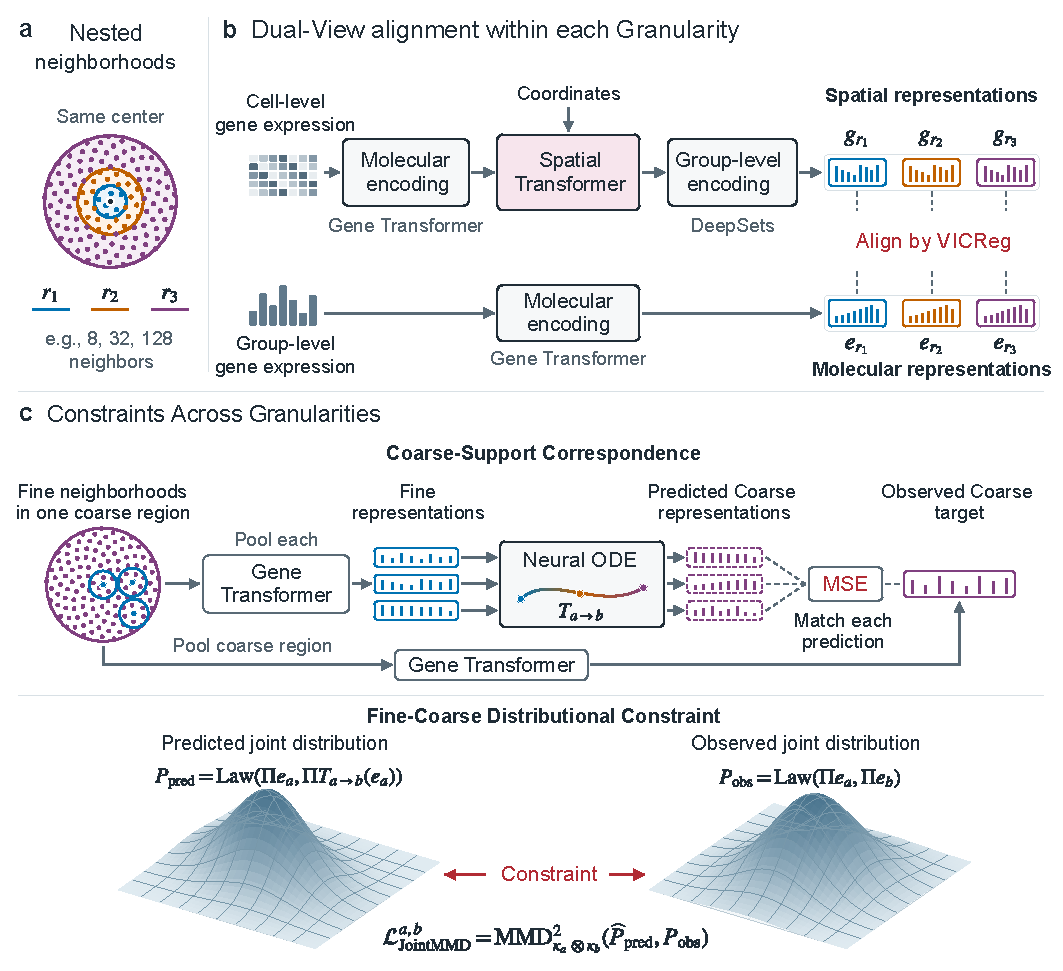
\includegraphics[width=\linewidth]{figures/zoomst_figure1_v5.pdf}
}
\caption{\textbf{ZoomST overview.}
\textbf{a}, Nested neighborhoods share a center and span increasing granularities, here 8, 32 and 128 measured positions.
\textbf{b}, Molecular and spatial encoders produce representations $e_r$ and $g_r$, aligned by VICReg within each granularity and retained for analysis.
\textbf{c}, A shared neural ODE predicts coarser molecular states. Coarse-support MSE compares predictions from fine observations with a common, directly encoded coarse target. Joint MMD compares fine--predicted-coarse pairs with fine--observed-coarse pairs at matched centers.}
\label{fig:method}
\end{figure}

\subsection{Observation granularity and nested tissue context}
\label{sec:nested-observations}

A tissue section contains expression profiles $x_i$ and coordinates $p_i$ at $N$ measured positions, each representing a cell or spatial bin. Let $S_{i,r}$ contain $i$ and its $r-1$ nearest spatial neighbors. The \emph{observation granularity} $r$ counts the positions summarized around $i$; increasing it expands context on the same measurement grid. Training uses nested supports at $r\in\Rset=\{8,32,128\}$. Their molecular profiles average preprocessed expression, $m_{i,r}=r^{-1}\sum_{j\in S_{i,r}}\bar x_j$. Expanding a support retains shared measurements and adds new context, providing paired observations without anatomical labels.

\subsection{Molecular--spatial representations within each granularity}
\label{sec:within-granularity}

The molecular view is $e_{i,r}=E_{\mathrm{PB}}(\operatorname{Tokenize}(m_{i,r}))\in\mathbb R^d$: a pseudobulk Transformer encodes gene identities and discretized expression values after pooling. The spatial view additionally describes arrangement. A position-wise Transformer supplies states $h_j$; a shared spatial Transformer contextualizes them using relative coordinates and a granularity identifier. A shared DeepSets readout~\citep{zaheer2017deepsets} pools the resulting states into $g_{i,r}\in\mathbb R^d$. Both views have $d=256$. The two molecular Transformers have separate parameters and share gene and expression-bin embeddings.

Masked expression reconstruction grounds both views in molecular content: $e_{i,r}$ and $g_{i,r}$ reconstruct the pooled neighborhood profile, alongside reconstruction of the focal observation. The combined reconstruction loss $\mathcal L_{\mathrm{rec}}$ and within-granularity VICReg alignment~\citep{bardes2022vicreg} define $\mathcal L_{\mathrm{base}}$. VICReg's variance and covariance terms regularize the aligned states. Both views remain available; transformations act on $e$, whose observation is the pooled molecular profile. Appendices~\ref{app:preprocessing} and~\ref{app:hyperparameters} specify tokenization, architecture and the base objective.

\subsection{Continuous Cross-Granularity Representation Transformation}
\label{sec:coarse-support}

To model how molecular representations change across spatial granularities, we parameterize a shared continuous transformation with a neural ODE~\citep{chen2018neuralode}. We define a normalized log-granularity coordinate $u(r)=\frac{\log_2(r/8)}{4}$, which maps the training granularities $r\in\{8,32,128\}$ to $0$, $\frac{1}{2}$, and $1$, respectively, so that equal multiplicative changes in neighborhood size correspond to equal intervals.

We define the continuous transformation from the molecular representation $e_{i,a}$ at source granularity $a$ to target granularity $b$ by integrating a learned vector field $f_\theta$ over the granularity coordinate,
\begin{equation}
\frac{dz(u)}{du}=f_\theta(z(u),u),\qquad
z(u(a))=e_{i,a},\qquad T_{a\to b}(e_{i,a})=z(u(b)).
\label{eq:granularity-ode}
\end{equation}
The shared vector field defines a continuous family of cross-granularity transformations rather than separate mappings for individual granularity pairs. It is implemented as a multilayer perceptron and initialized to zero so that training starts from identity transformations. We use fourth-order Runge--Kutta integration, with implementation details provided in Appendix~\ref{app:hyperparameters}.

\subsection{Soft distributional equivariance from nested observations}
\label{sec:granularity-supervision}

Rather than enforcing exact pointwise equality between transformed and directly encoded coarse states, we constrain their relationship statistically over matched locations:
\begin{equation}
\operatorname{Law}\bigl(Z_a,T_{a\to b}(Z_a)\bigr)
\;\approx\;\operatorname{Law}(Z_a,Z_b),
\label{eq:granularity-equivariance}
\end{equation}
where $(Z_a,Z_b)$ are directly encoded states at the same sampled location. Including the source preserves fine--coarse associations: shuffling coarse states changes their pairing while preserving their marginal distribution. Two complementary losses implement this relation: coarse-support correspondence aligns predictions from fine observations within each support to a common coarse target, while JointMMD matches fine--coarse associations across locations.

\paragraph{Coarse-support correspondence.}
A coarse support supplies a common target for fine descriptions centered within it. For $B$ focal centers, define $y_{i,b}=\stopgrad(e_{i,b})$, where $\stopgrad$ stops gradients, and $\Pset=\{(8,32),(8,128),(32,128)\}$. We minimize
\begin{equation}
\mathcal L_{\mathrm{CS}}
=\frac{1}{|\Pset|B}\sum_{(a,b)\in\Pset}\sum_{i=1}^{B}
\frac{1}{bd}\sum_{j\in S_{i,b}}
\left\|T_{a\to b}(e_{j,a})-y_{i,b}\right\|_2^2.
\label{eq:coarse-support-loss}
\end{equation}
Each $e_{j,a}$ is encoded around its own center $j$ and transformed separately. This loss aligns the mean prediction to the coarse target and reduces within-support dispersion. Supports, centers and granularity pairs receive equal weight at their respective averaging levels.

\paragraph{Joint association across locations.}
For a fixed orthogonal projection $\Pi:\mathbb R^{256}\to\mathbb R^{16}$, let $\widehat P_{ab}^{T,\Pi}$ and $\widehat P_{ab}^{\Pi}$ be the empirical distributions of $(\Pi e_{i,a},\Pi T_{a\to b}(e_{i,a}))$ and $(\Pi e_{i,a},\Pi e_{i,b})$ over the same centers. Their squared maximum mean discrepancy~\citep{gretton2012mmd} gives
\begin{equation}
\mathcal L_{\mathrm{JointMMD}}=\frac{1}{|\Pset|}\sum_{(a,b)\in\Pset}
\operatorname{MMD}_{\kappa_a\otimes\kappa_b}^2
\!\left(\widehat P_{ab}^{T,\Pi},\widehat P_{ab}^{\Pi}\right).
\label{eq:granularity-joint}
\end{equation}
The product of multibandwidth radial basis kernels compares source and destination jointly. Kernel source coordinates and observed targets are detached; gradients through predicted destinations update the transition and source encoder. Appendix~\ref{app:hyperparameters} gives the estimator and correspondence-loss decomposition.

\subsection{Pretraining and continuous granularity queries}
\label{sec:training-queries}

After base pretraining, we jointly optimize the encoders and transition on the same source sections with
\begin{equation}
\mathcal L=\mathcal L_{\mathrm{base}}+\lambda_{\mathrm{CS}}\mathcal L_{\mathrm{CS}}
+\lambda_{\mathrm{J}}\mathcal L_{\mathrm{JointMMD}}.
\label{eq:full-objective}
\end{equation}
The two cross-granularity weights warm up to one. Their inputs are clean molecular encodings; detached coarse targets come from the current encoder. All supervision uses 8, 32 and 128.

After training, the encoders and transition are frozen. Retained views support tissue analysis, while $\widehat e_i(r\mid a)=T_{a\to r}(e_{i,a})$ queries trained or unseen target ranges. From a common source $a_0$, the normalized response
\begin{equation}
R_i(a,b\mid a_0)=\frac{\|\widehat e_i(b\mid a_0)-\widehat e_i(a\mid a_0)\|_2}
{\sqrt d\,\log_2(b/a)}
\label{eq:granularity-response}
\end{equation}
measures predicted change per doubling of context. We use this normalized predicted change to compare relative context sensitivity across locations.

\section{Evaluation design}
\label{sec:experiments}

\paragraph{Pretraining and held-out evaluation.}
ZoomST is pretrained on 45 MOSTA mouse embryo sections~\citep{chen2022mosta}, with eight sections reserved in advance, one from each sampled stage from E9.5 to E16.5. Supervision uses only granularities 8, 32, and 128. Held-out representation and transformation tests freeze the encoders and transition; input preprocessing and target-fitted readouts follow Appendices~\ref{app:preprocessing} and~\ref{app:dual-view}. The No Cross ablation omits cross-granularity supervision with the same total number of training updates. Held-out tests evaluate generalization, matched continuations analyze the training objectives, and source-section anatomical cases interpret granularity-dependent representations and responses. Table~\ref{tab:evaluation_protocol} specifies data use for each analysis.

\paragraph{Retained tissue information and correspondence.}
Whole-section clustering compares frozen ZoomST, Novae, and SToFM with target-fitted GraphST, BANKSY, MENDER, and STAGATE, sharing positions, annotation-defined cluster counts, and downstream readouts with the stated method-specific preprocessing. AMI and physical 32-neighbor retention measure anatomical and local spatial organization. Stage-balanced Brain observations from the held-out sections evaluate developmental ordering by diffusion-pseudotime--stage correlations (Appendix~\ref{app:developmental-ordering}). Separately, equal-update continuations on three sections compare Base, Base+CS, and Base+CS+JointMMD on their respective adapted sections. Native neighbor overlap and same-location Recall@32 measure molecular-state correspondence without a fitted transformation (Appendix~\ref{app:objective-ablation}).

\paragraph{Transformation and response generalization.}
Direct neighborhood encodings provide reference targets. Trained-pair state prediction uses all held-out positions; joint-association tests include shuffled-pair controls and projections unused in training. Unseen-target prediction uses 1,024 fixed positions per section at granularities 12, 16, 24, 48, 64, and 96. These target encodings do not enter training or prediction. The same held-out locations evaluate response ordering over four doubling intervals (Appendices~\ref{app:granularity-transfer} and~\ref{app:scale-continuum}).

\paragraph{Anatomical interpretation.}
Matched IoU readouts compare Lung and Smooth muscle at fine and coarse granularities. Facial nerve and Brain response analyses compare predicted change with encoded change and annotated neighborhood composition. These anatomical cases use E14.5 E1S1 and E16.5 E1S1 from the training set; the Brain mapping display uses held-out E16.5 E2S13. Physical extents use the exact nested supports and nominal bin50 calibration. Sampling, domains, and response definitions are specified in Appendices~\ref{app:scale-cases} and~\ref{app:response-meaning}.

\section{Results}
\label{sec:results}

We evaluate two outcomes of cross-granularity pretraining: the tissue information retained in each representation and the predictive relationships learned between representations. We first establish anatomical transfer to held-out sections, then examine how relational supervision enriches developmental information and organizes correspondence without making the granularities interchangeable. We finally test transformations at trained and unseen target granularities and use their predicted responses to characterize spatial context dependence.

\subsection{Frozen representations recover anatomy in held-out sections}
\label{sec:dual-view-identification}

Frozen ZoomST representations distinguish anatomical compartments on sections excluded from pretraining. We compare whole-section clustering with atlas annotations across all eight held-out MOSTA sections. Molecular features concatenate $e_8,e_{32},e_{128}$, spatial features concatenate $g_8,g_{32},g_{128}$, and joint features combine both views. All pretrained encoders remain frozen; the target-section readouts are specified in Appendix~\ref{app:dual-view}.

Joint ZoomST features achieve higher AMI than the evaluated public pretrained baselines on every held-out section, with an equal-section mean of 0.577, and remain competitive with target-fitted spatial methods (Table~\ref{tab:representation-summary}). The same features retain 52.7\% of physical 32-nearest neighbors on average, linking anatomical agreement to local spatial organization. The matched-update No Cross model has similar mean AMI (0.575), but lower neighbor retention (50.4\%). Thus, the full model retains anatomical discrimination while improving local spatial correspondence relative to this ablation.

\begin{table}[!htbp]
\centering\small
\caption{\textbf{Tissue mapping and neighbor retention on eight held-out MOSTA sections.} \textbf{(a)} AMI as mean $\pm$ sample SD over clustering seeds 42, 43, and 44; the summary averages sections equally within each seed. \textbf{(b)} Equal-section mean recovery of physical 32-nearest neighbors. Molecular and Spatial Views each concatenate three granularities; Joint combines both. No Cross uses the same joint readout and total training updates without cross-granularity supervision. Pretrained encoders are frozen. Bold marks the top three unrounded values per row, including third-place ties. Protocol: Appendix~\ref{app:dual-view}.}
\label{tab:representation-summary}
\label{tab:dual-view-sections}
\setlength{\tabcolsep}{0.8pt}
\renewcommand{\arraystretch}{1.05}
\begin{tabular}{lcccccccccc}
\toprule
 & \multicolumn{4}{c}{ZoomST Versions} & \multicolumn{2}{c}{Frozen pretrained} & \multicolumn{4}{c}{Target-fitted} \\
\cmidrule(lr){2-5}\cmidrule(lr){6-7}\cmidrule(lr){8-11}
Stage & Joint & \shortstack{Molecular\\View} & \shortstack{Spatial\\View} & \shortstack{No Cross\\Ablation} & Novae & SToFM & GraphST & BANKSY & MENDER & STAGATE \\
\midrule
\multicolumn{11}{l}{\textbf{(a) Anatomical agreement: AMI} $\uparrow$} \\
E9.5 & \textbf{0.547} & 0.486 & \textbf{0.556} & 0.533 & 0.371 & 0.211 & 0.538 & 0.540 & 0.530 & \textbf{0.556} \\
 & {\scriptsize $\pm 0.014$} & {\scriptsize $\pm 0.016$} & {\scriptsize $\pm 0.017$} & {\scriptsize $\pm 0.005$} & {\scriptsize $\pm 0.007$} & {\scriptsize $\pm 0.004$} & {\scriptsize $\pm 0.009$} & {\scriptsize $\pm 0.021$} & {\scriptsize $\pm 0.005$} & {\scriptsize $\pm 0.028$} \\
\addlinespace[2pt]
E10.5 & \textbf{0.549} & 0.516 & 0.534 & \textbf{0.549} & 0.390 & 0.262 & 0.534 & 0.539 & 0.531 & \textbf{0.544} \\
 & {\scriptsize $\pm 0.009$} & {\scriptsize $\pm 0.014$} & {\scriptsize $\pm 0.002$} & {\scriptsize $\pm 0.004$} & {\scriptsize $\pm 0.004$} & {\scriptsize $\pm 0.013$} & {\scriptsize $\pm 0.010$} & {\scriptsize $\pm 0.013$} & {\scriptsize $\pm 0.001$} & {\scriptsize $\pm 0.023$} \\
\addlinespace[2pt]
E11.5 & \textbf{0.628} & \textbf{0.608} & \textbf{0.615} & 0.602 & 0.444 & 0.291 & 0.502 & 0.573 & 0.561 & 0.559 \\
 & {\scriptsize $\pm 0.001$} & {\scriptsize $\pm 0.004$} & {\scriptsize $\pm 0.010$} & {\scriptsize $\pm 0.001$} & {\scriptsize $\pm 0.008$} & {\scriptsize $\pm 0.007$} & {\scriptsize $\pm 0.004$} & {\scriptsize $\pm 0.022$} & {\scriptsize $\pm 0.002$} & {\scriptsize $\pm 0.007$} \\
\addlinespace[2pt]
E12.5 & \textbf{0.613} & \textbf{0.614} & 0.607 & \textbf{0.618} & 0.447 & 0.307 & 0.509 & 0.583 & 0.582 & 0.585 \\
 & {\scriptsize $\pm 0.015$} & {\scriptsize $\pm 0.003$} & {\scriptsize $\pm 0.006$} & {\scriptsize $\pm 0.013$} & {\scriptsize $\pm 0.011$} & {\scriptsize $\pm 0.008$} & {\scriptsize $\pm 0.017$} & {\scriptsize $\pm 0.007$} & {\scriptsize $\pm 0.009$} & {\scriptsize $\pm 0.017$} \\
\addlinespace[2pt]
E13.5 & \textbf{0.578} & 0.541 & \textbf{0.579} & 0.573 & 0.432 & 0.334 & 0.386 & \textbf{0.593} & 0.573 & 0.544 \\
 & {\scriptsize $\pm 0.012$} & {\scriptsize $\pm 0.011$} & {\scriptsize $\pm 0.012$} & {\scriptsize $\pm 0.003$} & {\scriptsize $\pm 0.003$} & {\scriptsize $\pm 0.017$} & {\scriptsize $\pm 0.013$} & {\scriptsize $\pm 0.015$} & {\scriptsize $\pm 0.009$} & {\scriptsize $\pm 0.006$} \\
\addlinespace[2pt]
E14.5 & 0.563 & 0.556 & 0.558 & \textbf{0.571} & 0.450 & 0.407 & 0.453 & \textbf{0.572} & 0.535 & \textbf{0.579} \\
 & {\scriptsize $\pm 0.019$} & {\scriptsize $\pm 0.009$} & {\scriptsize $\pm 0.006$} & {\scriptsize $\pm 0.017$} & {\scriptsize $\pm 0.009$} & {\scriptsize $\pm 0.006$} & {\scriptsize $\pm 0.005$} & {\scriptsize $\pm 0.008$} & {\scriptsize $\pm 0.004$} & {\scriptsize $\pm 0.021$} \\
\addlinespace[2pt]
E15.5 & \textbf{0.626} & \textbf{0.625} & 0.614 & \textbf{0.630} & 0.494 & 0.405 & 0.422 & 0.614 & 0.600 & 0.604 \\
 & {\scriptsize $\pm 0.001$} & {\scriptsize $\pm 0.006$} & {\scriptsize $\pm 0.004$} & {\scriptsize $\pm 0.013$} & {\scriptsize $\pm 0.004$} & {\scriptsize $\pm 0.005$} & {\scriptsize $\pm 0.005$} & {\scriptsize $\pm 0.003$} & {\scriptsize $\pm 0.010$} & {\scriptsize $\pm 0.003$} \\
\addlinespace[2pt]
E16.5 & 0.513 & 0.497 & \textbf{0.532} & 0.524 & 0.449 & 0.331 & 0.403 & \textbf{0.526} & 0.509 & \textbf{0.540} \\
 & {\scriptsize $\pm 0.010$} & {\scriptsize $\pm 0.012$} & {\scriptsize $\pm 0.007$} & {\scriptsize $\pm 0.008$} & {\scriptsize $\pm 0.006$} & {\scriptsize $\pm 0.007$} & {\scriptsize $\pm 0.002$} & {\scriptsize $\pm 0.006$} & {\scriptsize $\pm 0.016$} & {\scriptsize $\pm 0.006$} \\
\addlinespace[2pt]
Mean AMI & \textbf{0.577} & 0.555 & \textbf{0.574} & \textbf{0.575} & 0.435 & 0.319 & 0.468 & 0.567 & 0.553 & 0.564 \\
 & {\scriptsize $\pm 0.004$} & {\scriptsize $\pm 0.006$} & {\scriptsize $\pm 0.003$} & {\scriptsize $\pm 0.003$} & {\scriptsize $\pm 0.001$} & {\scriptsize $\pm 0.003$} & {\scriptsize $\pm 0.003$} & {\scriptsize $\pm 0.003$} & {\scriptsize $\pm 0.002$} & {\scriptsize $\pm 0.0005$} \\
\addlinespace[2pt]
\midrule
\multicolumn{11}{l}{\textbf{(b) Local spatial organization} $\uparrow$} \\
\shortstack{Neighbor\\retention} & \textbf{0.527} & 0.502 & \textbf{0.523} & \textbf{0.504} & 0.313 & 0.033 & 0.268 & 0.483 & 0.354 & 0.354 \\
\bottomrule
\end{tabular}

\end{table}

The held-out E16.5 E2S13 Brain case illustrates the complementary information in the two views (Figure~\ref{fig:dual-view-brain}). Molecular features recover most Brain positions but include neighboring tissue; spatial features make fewer extra assignments but miss part of the Brain. Joint features reduce this tradeoff, increasing Brain IoU from 0.884 for $e$ and 0.905 for $g$ to 0.962. Whole-section maps and section-wise spatial retention are provided in Figures~\ref{fig:dual-view-e125} and~\ref{fig:dual-view-retention}. These results establish a transferable representation base from which to assess the additional value of learning granularity relationships.

\begin{figure}[!htbp]
\centering
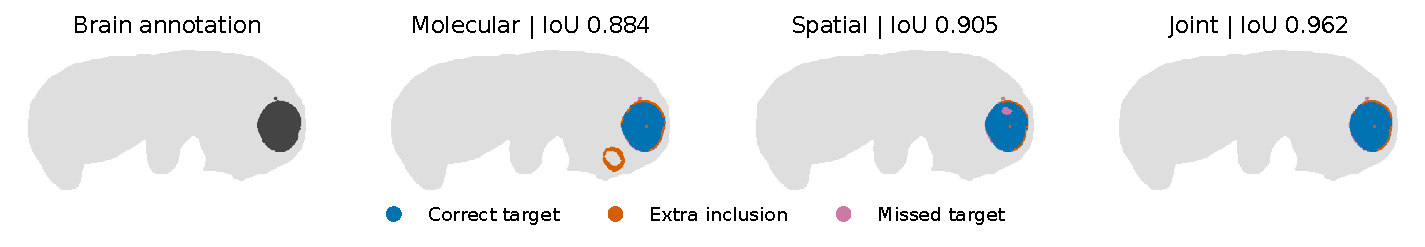
\includegraphics[width=\linewidth]{figures/brain_complementarity.pdf}
\caption{\textbf{Complementary molecular and spatial errors on a held-out section.} Annotation, molecular, spatial, and joint Brain assignments in E16.5 E2S13. Blue: correct assignments; orange: extra assignments; magenta: missed Brain. All maps use the same whole-section readout and seed 42. Each feature set combines its respective training granularities.}
\label{fig:dual-view-brain}
\end{figure}
\FloatBarrier

\subsection{Cross-granularity learning enriches developmental information}
\label{sec:developmental-information}

Having examined the two views in zero-shot tissue mapping, we next ask what cross-granularity learning adds to the retained representations. We compare the final ZoomST and No Cross checkpoints in an equal-budget controlled ablation. No Cross retains within-granularity learning and omits cross-granularity supervision. With both encoders frozen, we evaluate Joint separately at granularities 8, 32, and 128 on held-out MOSTA and HESTA sections, using independently pretrained mouse and human models (Appendix~\ref{app:preprocessing}).

Fine-granularity AMI improves on seven of eight held-out MOSTA sections and all seven HESTA sections (Table~\ref{tab:cross-granularity-ami}a). These AMI gains are modest, prompting us to ask whether the learned relations add information about developmental progression within the same tissue.


We examine Brain through two complementary tasks: developmental ordering and stage prediction. Diffusion pseudotime assesses agreement with the observed developmental sequence through spot-level Spearman correlation. A linear readout tests whether stage can be predicted from frozen representations, training on other sections and evaluating an entire held-out section. Together, these tasks measure unsupervised ordering and the stage information accessible to a supervised readout (Appendix~\ref{app:developmental-ordering}).

The developmental gains are particularly evident in coarse representations (Table~\ref{tab:cross-granularity-development}b). MOSTA shows its largest ordering improvement at the coarsest granularity, where spot-level correlation changes from negative to positive. HESTA shows higher spot-level correlations at every granularity. Stage-prediction error decreases at every granularity in both atlases, with the largest relative MAE reductions at $k=128$: 21.01\% on MOSTA and 8.73\% on HESTA. On MOSTA, adding JointMMD further reduces stage-prediction error relative to CS alone at all three granularities (Appendix~\ref{app:objective-ablation}). Cross-granularity learning thus enriches developmental information within broad tissue contexts, beyond its modest effect on anatomical clustering.

\begin{table}[!htbp]
\centering
\caption{\textbf{Cross-granularity learning across mouse and human atlases.} \textbf{(a)} Joint AMI, with SD over downstream clustering initializations below each mean; sections are averaged equally within each clustering run. Improved counts held-out sections with higher mean AMI. \textbf{(b)} Brain spot-level DPT correlation and leave-one-section-out stage MAE, in embryonic days for MOSTA and Carnegie stages for HESTA. Bold marks the better paired value, including ties. Evaluation protocols: Appendix~\ref{app:dual-view}--\ref{app:developmental-ordering}.}
\label{tab:cross-granularity-ami}
\label{tab:cross-granularity-development}
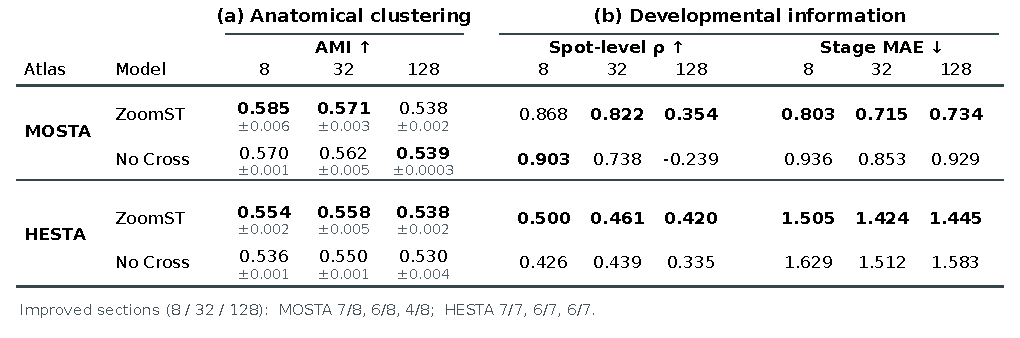
\includegraphics[width=\linewidth]{figures/cross_granularity_combined.pdf}
\end{table}
\FloatBarrier

This developmental information also gives ZoomST an advantage in cross-method comparisons (Figure~\ref{fig:developmental-ordering}). Combining all three granularities, ZoomST achieves the highest spot-level correlation on both MOSTA and HESTA among methods with complete-stage readouts. The ablation and cross-method results show that learning relations across granularities strengthens the developmental content of tissue representations while preserving their anatomical utility.

\begin{figure}[!htbp]
\centering
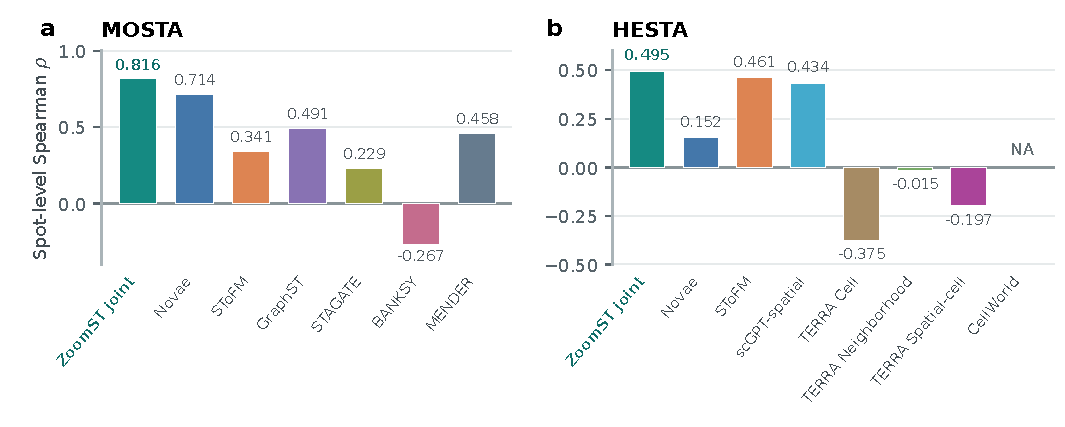
\includegraphics[width=0.98\linewidth]{figures/developmental_ordering_spearman.pdf}
\caption{\textbf{Developmental ordering on MOSTA and HESTA Brain.} Methods share observations and a fixed root within each atlas: (a) MOSTA, 4,712 spots; (b) HESTA, 2,560 spots. ZoomST combines Joint features from three granularities. NA: CellWorld does not connect CS18 to the root. Baseline fitting and DPT settings: Appendix~\ref{app:developmental-ordering}.}
\label{fig:developmental-ordering}
\end{figure}
\FloatBarrier

\subsection{Granularity-specific anatomical uses}
\label{sec:objective-ablation}

\label{sec:anatomical-scale-preference}
The retained granularities favor different anatomical regions. We compare ZoomST Spatial representations at granularities 8, 32, and 128 with six external methods across all 43 regions in the eight held-out sections. For each section, all methods share annotation-balanced clustering-fit positions and are scored on the full section by region-wise IoU (Appendix~\ref{app:region-scale}). Table~\ref{tab:regional-spatial-iou} highlights two patterns from the complete benchmark in Table~\ref{tab:regional-spatial-iou-full}. Locally homogeneous Spinal cord, Kidney, and Olfactory epithelium favor granularity 128, whereas boundary-rich Mucosal epithelium, Blood vessel, and Surface ectoderm favor granularity 8. Spinal cord IoU rises from 0.390 at granularity 8 to 0.489 at 128, while Blood vessel falls from 0.347 to 0.138. In these examples, the preferred ZoomST granularity also exceeds all six external methods. The choice of context therefore changes which anatomical structures the representation resolves best.

These scale preferences track the composition of the surrounding tissue. We measure neighborhood homogeneity by the mean same-label fraction among 128 spatial neighbors, and boundary fraction by the proportion of positions with at least one differently labeled neighbor among their eight nearest neighbors. Across 137 section--region observations, the coarse-scale gain, $\Delta\mathrm{IoU}=\mathrm{IoU}_{128}-\mathrm{IoU}_{8}$, increases with homogeneity and decreases with boundary fraction (Figure~\ref{fig:region-geometry}). The mean within-section Spearman correlations are 0.409 and $-0.337$, respectively, with each direction observed in seven of eight sections. Locally homogeneous structures therefore tend to benefit more from broad context, while regions with frequent boundaries favor finer context. The representations thus retain distinct anatomical uses after cross-granularity learning.

\begin{figure}[!htbp]
\centering
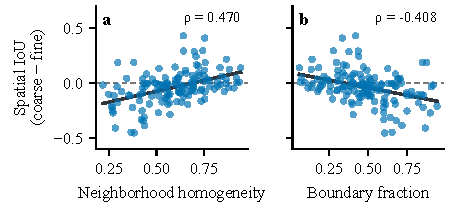
\includegraphics[width=\linewidth]{figures/region_geometry.pdf}
\caption{\textbf{Coarse-scale anatomical gains track neighborhood homogeneity and boundary frequency.} Each point is one of 137 section--region observations from eight held-out sections; colors and symbols identify developmental stages. The vertical axis is the Spatial IoU difference between granularities 128 and 8, in percentage points, after averaging three clustering seeds. Positive values favor coarse context. (a) Mean same-label fraction among 128 spatial neighbors. (b) Fraction of positions with a differently labeled neighbor among eight spatial neighbors. Geometry uses the full measured section, excluding each focal position from its own neighbor set. Solid lines show pooled linear fits; dashed lines mark equal IoU. The panels report pooled Spearman correlations and the mean of eight within-section correlations.}
\label{fig:region-geometry}
\end{figure}
\FloatBarrier
\input{tables/region_spatial_iou}

\FloatBarrier

\subsection{Learned transformations generalize to new sections and granularities}
\label{sec:granularity-transfer}
\label{sec:scale-continuum}

The preceding results concern directly encoded representations. We now ask whether the learned relationships themselves support prediction, first at trained target granularities on new sections and then at intermediate granularities absent from training. In both tests, a prediction uses only the source molecular state and the requested granularity. Direct encodings of the actual target neighborhoods provide the scoring references.

\paragraph{Trained relationships transfer to held-out sections.}
Across all eight held-out sections, transformed states have lower target MSE than unchanged fine states for each trained granularity pair (Figure~\ref{fig:generalization-summary}A). Equal-section mean reductions are 21.3\%, 27.0\%, and 11.8\% for $8\to32$, $8\to128$, and $32\to128$, respectively. Correct fine--predicted-coarse pairings also have lower joint-distribution discrepancy than shuffled pairings in every section and direction, including evaluation with projections unused in training (Figure~\ref{fig:generalization-summary}B). Shuffling preserves the predicted coarse marginal distribution but disrupts its association with the fine source. Together, the error reduction and pairing control support transferable, location-dependent fine--coarse relationships (Appendix~\ref{app:granularity-transfer}).

\paragraph{Discrete supervision supports unseen-granularity queries.}
With both encoder and transition frozen after training only at 8, 32, and 128, we query six unseen granularities---12, 16, 24, 48, 64, and 96---from the same $e_{i,8}$. Predictions reduce target MSE in all 48 held-out section--granularity conditions (Figure~\ref{fig:generalization-summary}A). Averaging prediction and unchanged-source errors over the six targets within each section, then averaging the section-level relative reductions, gives a 21.96\% reduction. Intermediate encodings are used only for evaluation. The same learned transformation can therefore predict descriptions at observation ranges beyond the discrete training set; all section-level errors and the separate PCA illustrations are provided in Appendix~\ref{app:unseen-state-detail}.

\begin{figure}[!htbp]
\centering
\begin{minipage}[t]{0.625\linewidth}
\centering\vspace{0pt}
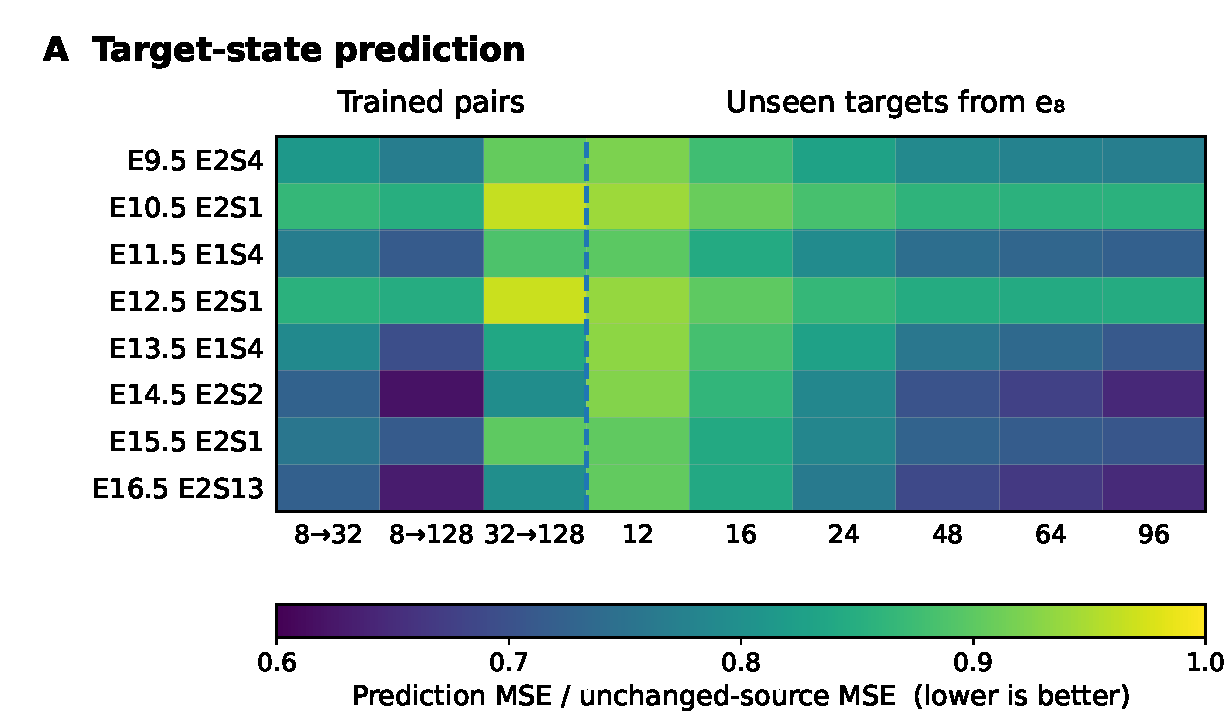
\includegraphics[width=\linewidth]{figures/results_generalization_matrix.pdf}
\end{minipage}\hfill
\begin{minipage}[t]{0.355\linewidth}
\centering\vspace{0pt}
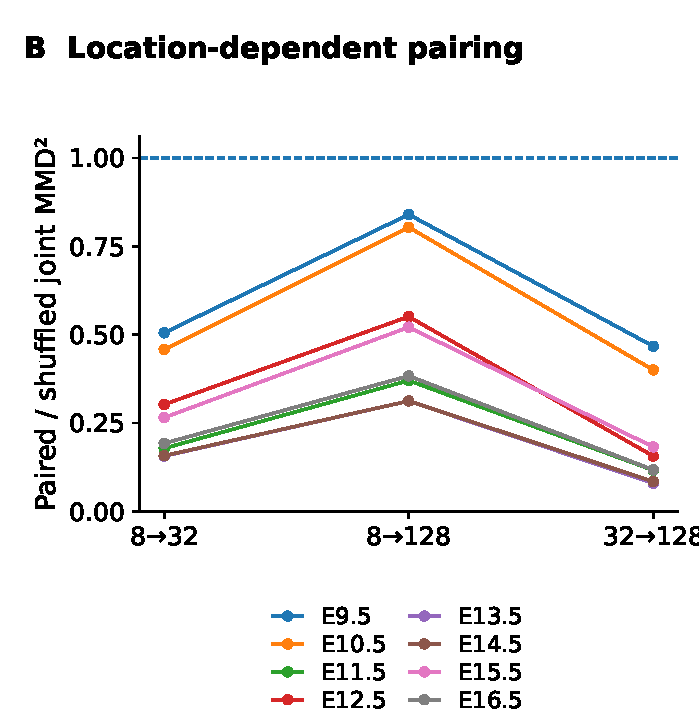
\includegraphics[width=\linewidth]{figures/results_pairing_control.pdf}
\end{minipage}
\caption{\textbf{Transformation generalization across held-out sections and observation granularities.} \textbf{A}, Target-MSE ratios for the three trained source--target pairs (left) and six unseen targets queried from $e_8$ (right). Each cell compares prediction with an unchanged source against the same directly encoded target. Trained-pair evaluation uses all section positions; unseen-target evaluation uses 1,024 fixed positions per section. All 24 trained-pair and 48 unseen-target ratios are below one. \textbf{B}, Correct-pair to shuffled-pair joint-MMD ratios for the trained pairs, averaged over four batches and eight projections unused in training. Each line is one held-out section. Values are from Tables~\ref{tab:granularity-transfer-sections} and~\ref{tab:ode-intermediate-sections}.}
\label{fig:generalization-summary}
\end{figure}

\paragraph{Continuous parameterization improves a matched prediction task.}
In a separate comparison on a shared frozen encoder, the neural ODE reduces mean unseen-granularity MSE by 10.86\% relative to a granularity-conditioned residual MLP, with lower error on all eight held-out sections. Both heads use the same source states and encoded targets (Appendix~\ref{app:transition-comparison}). This matched comparison supports the continuous parameterization; the preceding held-out tests establish the predictive capability of the jointly trained model.
\FloatBarrier

\subsection{Predicted responses reveal relative spatial context sensitivity}
\label{sec:context-response}

Once a transformation predicts states at different observation ranges, their differences can be used to compare context dependence across locations. We evaluate the normalized response in Equation~\ref{eq:granularity-response} against directly encoded changes over the same intervals, with all predictions starting from a common $e_8$.

\paragraph{Predicted response orders context-sensitive locations.}
For each held-out section and each of four doubling intervals, we rank 1,024 locations by predicted response and compare the highest and lowest quarters. The high-response quarter has a larger mean directly encoded change in 31 of 32 section--interval conditions (Figure~\ref{fig:heldout-response-ordering}). Equal-section mean high-to-low ratios range from 1.440 to 1.673 across the four intervals. Predicted response thus identifies relative differences in how strongly tissue descriptions depend on observation range (Appendix~\ref{app:response-meaning}).

\begin{figure}[!htbp]
\centering
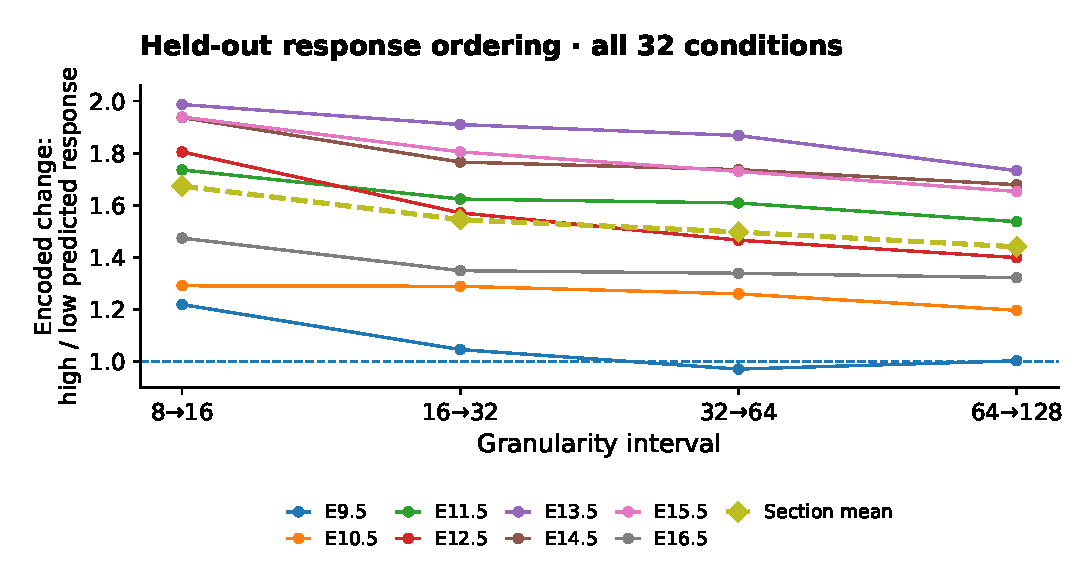
\includegraphics[width=0.78\linewidth]{figures/results_response_ordering.pdf}
\caption{\textbf{Predicted response identifies larger encoded changes on held-out sections.} Locations are ranked separately within each section and interval by predicted finite response. The ordinate is the ratio of mean directly encoded change in the highest versus lowest predicted-response quarter, with 256 locations per group. All 32 section--interval conditions are shown; 31 are above one. Lines denote sections and diamonds denote equal-section means. Full values: Table~\ref{tab:ode-response-heldout}.}
\label{fig:heldout-response-ordering}
\end{figure}

\paragraph{Anatomical context gives the response an interpretation.}
Two source-section cases illustrate distinct forms of context dependence. In E14.5 E1S1 Facial nerve, predicted and directly encoded changes correlate over $64\to128$ across all 64 locations ($\rho=0.791$; Figure~\ref{fig:scale-continuum}C). Predicted response also correlates with changes in annotated neighbor composition ($\rho=0.707$; Figure~\ref{fig:ode-context}A). In the highest-response quarter, the mean nerve fraction falls from 71.4\% to 45.7\% as context expands, compared with 43.4\% to 36.2\% in the lowest quarter (Figure~\ref{fig:ode-context}B). High-response locations therefore undergo a larger transition from a nerve-dominated neighborhood to surrounding tissue; low-response locations already include substantial surrounding tissue at the smaller range.

In E16.5 E1S1 Brain, context can change even when a broad annotation does not. Over $8\to16$, 95 sampled locations have only Brain-labeled neighbors at both granularities, yet their predicted and directly encoded responses correlate at $\rho=0.645$ (Appendix~\ref{app:response-meaning}). The response therefore captures molecular-context variation within a broad anatomical label as well as shifts in tissue composition. Whole-section maps illustrate the spatial heterogeneity of this dependence (Figure~\ref{fig:ode-context}C,D).

\begin{figure}[H]
\centering
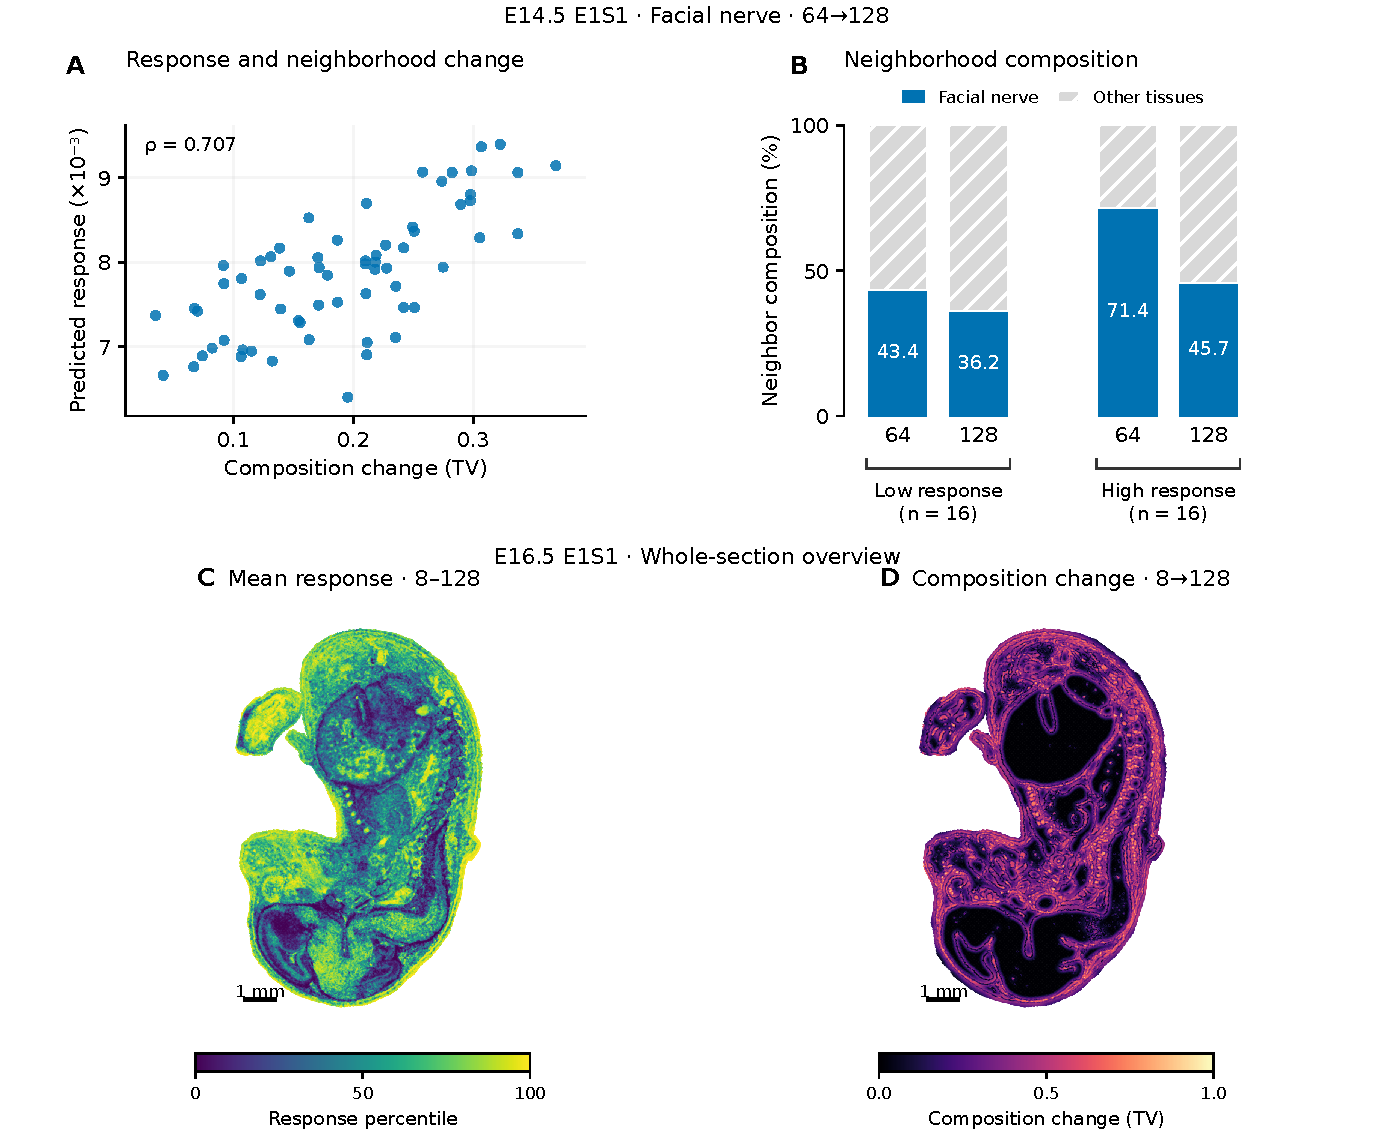
\includegraphics[width=0.92\linewidth]{figures/response_and_neighborhood_context.pdf}
\caption{\textbf{Context response distinguishes different dependencies on surrounding tissue.} \textbf{A}, Predicted finite response versus annotation-composition change (total variation, TV) at all 64 E14.5 E1S1 Facial nerve locations over $64\to128$. \textbf{B}, Mean composition at 64 and 128 for the lowest and highest response quarters, following the same 16 locations per group. \textbf{C,D}, E16.5 E1S1 whole-section maps of path-averaged instantaneous response over 8--128 (percentiles) and observed composition change from 8 to 128. These are spatial overviews of different quantities. All 121,767 locations are retained without smoothing. Both sections are anatomical cases from the training set; predictions start from fixed $e_8$. Scale bars: 1\,mm. Definitions: Appendix~\ref{app:response-meaning}.}
\label{fig:ode-context}
\end{figure}

\FloatBarrier

\section{Discussion and conclusion}

ZoomST makes observation granularity an explicit variable in spatial transcriptomic pretraining by jointly learning granularity-specific tissue representations and transformations between them. Its design combines molecular--spatial dual-view alignment within each granularity with soft distributional equivariance across nested neighborhoods. A shared neural ODE learns continuous transformations from supervision at discrete granularities, while the representations at each granularity remain separately usable. Different neighborhood extents favor different tissue structures; across the held-out MOSTA sections, finer contexts yield higher overall anatomical agreement, while coarser contexts retain more physical neighbors. The scale-specific comparison with the matched-update No Cross ablation shows that learning cross-granularity transformations enriches developmental-stage ordering in coarse joint representations while retaining comparable tissue-identification performance. Learned relations between observation scales thus help broad-context embeddings retain information about developmental progression alongside tissue identity and local spatial organization.

The learned transformations also predict directly encoded coarse and unseen intermediate states. Across held-out MOSTA sections, predicted responses generally track relative differences in encoded change, with anatomical analyses linking these differences to neighborhood composition. This makes observation granularity both a source of self-supervision and an axis for tissue analysis.

\clearpage
\setlength{\textfloatsep}{10pt plus 2pt minus 2pt}
\setlength{\floatsep}{8pt plus 2pt minus 2pt}
\setlength{\intextsep}{8pt plus 2pt minus 2pt}
\section{Reproducibility Statement}
The appendices specify data splits, preprocessing, model architecture, optimization, and evaluation protocols. Reported figures and tables are derived from saved model outputs using the stated readouts. Downstream K-means clustering is repeated with three seeds: 42, 43, and 44.

\section{Ethics Statement}
This work uses published MOSTA mouse embryo and HESTA human embryo spatial-transcriptomics data and their associated anatomical labels, following the original data access and use conditions. The model is intended for biological research.

\section{AI-Use Disclosure}
Generative AI tools assisted with language polishing, translation, and consistency checks across the text, figures, tables, and reported results. They also supported literature searches and code preparation. The authors retain responsibility for the final manuscript and all reported findings.


\bibliography{references}
\bibliographystyle{iclr2027_conference}

\clearpage
\appendix
\numberwithin{figure}{section}
\numberwithin{table}{section}
\renewcommand{\thefigure}{\thesection\arabic{figure}}
\renewcommand{\thetable}{\thesection\arabic{table}}
\renewcommand{\theHfigure}{appendix.\thesection.\arabic{figure}}
\renewcommand{\theHtable}{appendix.\thesection.\arabic{table}}
\section{Data and preprocessing}
\label{app:preprocessing}

\paragraph{Data split.}
MOSTA supplies 53 mouse embryo sections. We reserved one section from each developmental stage from E9.5 to E16.5 in advance for evaluation and used the remaining 45 sections for pretraining. Training spans the same eight stages. Table~\ref{tab:heldout-inventory} lists the held-out sections; Table~\ref{tab:evaluation_protocol} summarizes data use and aggregation for each analysis.

\begin{table}[!htbp]
\centering\small
\caption{\textbf{Held-out section inventory.} Every listed section is excluded from both pretraining stages.}
\label{tab:heldout-inventory}
\begin{tabular}{ll}
\toprule
Stage & Held-out section \\
\midrule
E9.5 & E9.5 E2S4 \\
E10.5 & E10.5 E2S1 \\
E11.5 & E11.5 E1S4 \\
E12.5 & E12.5 E2S1 \\
E13.5 & E13.5 E1S4 \\
E14.5 & E14.5 E2S2 \\
E15.5 & E15.5 E2S1 \\
E16.5 & E16.5 E2S13 \\
\bottomrule
\end{tabular}
\end{table}

\paragraph{Input preprocessing.}
The inputs use the original \texttt{count} layer and a 30,235-entry gene vocabulary. Existing center tokens are inherited from the prepared source data. Neighborhood profiles average normalized expression over the full gene space before selecting up to 512 tokens and assigning 31 nonzero expression bins, with bin zero reserved for padding. The inherited preprocessing uses library normalization to $10^4$, $\log(1+x)$, and section-specific nonzero gene medians; genes with fewer than ten nonzero observations use a fallback median. Target sections supply their own gene statistics and use the inherited vocabulary. Whole-section readout standardization, PCA, and clustering are fitted on target-section positions; method-specific settings are given in Appendix~\ref{app:dual-view}.

Relative coordinates are centered at the focal position and scaled by the maximum distance within its 128-neighbor window, then sliced to smaller supports. Granularity counts observations; its physical extent depends on the sampled tissue. Maps preserve the measured lattice and leave missing positions empty, without label interpolation.

\begin{table}[!htbp]
\centering\small
\caption{\textbf{Data split and evaluation protocol.} These conditions apply to the corresponding evaluations throughout the paper.}
\label{tab:evaluation_protocol}
\begin{tabularx}{\linewidth}{@{}p{0.20\linewidth}X@{}}
\toprule
Evaluation & Data use and aggregation \\
\midrule
Held-out sections & The eight sections in Table~\ref{tab:heldout-inventory} evaluate pretrained encoders with frozen weights. Input preprocessing and target-fitted readouts are specified above and in Appendix~\ref{app:dual-view}. \\
Anatomical analyses & E14.5 E1S1 (granularity and Facial nerve analyses) and E16.5 E1S1 (state and context-response analyses) belong to the training set. The E12.5 E2S1 whole-section map and E16.5 E2S13 Brain mapping display use held-out sections. \\
Developmental ordering & Stage-balanced Brain observations from the held-out sections evaluate pseudotime--stage agreement. Sampling, shared baseline fits, and both correlation readouts are specified in Appendix~\ref{app:developmental-ordering}. \\
Response summaries & Direct-encoding analyses use eight training E1S1 sections and eight holdouts. Section--domain--range summaries combine both groups; the high--low response comparison reports the eight holdouts separately. \\
Matched continuation & E12.5 E2S1, E14.5 E1S1, and E16.5 E1S1 are adapted separately and evaluated on the respective adapted section, using one training seed. E12.5 was excluded from base pretraining; the other two sections were included. \\
Aggregation & Section summaries receive equal weight. Position-level distributions describe within-section variation; queries, projections, shuffles and batches specify sampling and numerical averaging. \\
\bottomrule
\end{tabularx}
\end{table}

\paragraph{External pretrained models.}
Novae uses the public mouse-0 weights, and SToFM uses its public checkpoint with the specified mouse-to-human gene mapping. The sections held out from ZoomST training appear in the SToCorpus-88M inventory, so SToFM may have been exposed to our zero-shot evaluation data.

\section{Architecture and optimization}
\label{app:hyperparameters}

\subsection{Backbone and within-granularity learning}

Both representation views have width 256. The position-wise and pseudobulk encoders each use two Transformer layers and eight attention heads, with separate Transformer parameters and shared gene and expression-bin embeddings. The spatial-context Transformer has four layers and eight attention heads and is shared across granularities. The DeepSets maps $\phi$ and $\rho$ each use layer normalization and a two-layer multilayer perceptron with hidden width 512, GELU activation, and dropout 0.1. The same maps are applied at each granularity.

For clarity, the pooled profile and spatial set readout are
\begin{equation}
m_{i,r}=r^{-1}\sum_{j\in S_{i,r}}\bar x_j,\qquad
 g_{i,r}=\rho\!\left(r^{-1}\sum_{j\in S_{i,r}}\phi(H_{ij,r})\right).
\label{eq:neighborhood-profile}
\end{equation}
The base objective combines reconstruction with same-support view alignment:
\begin{equation}
\mathcal L_{\mathrm{base}}=\mathcal L_{\mathrm{rec}}+
\frac{\lambda_{\mathrm{view}}}{|\Rset|}\sum_{r\in\Rset}\mathcal L_{\mathrm{VICReg}}(e_r,g_r).
\label{eq:base-objective}
\end{equation}
Here $e_r,g_r$ collect the sampled centers at granularity $r$.

The molecular view averages preprocessed expression over the neighborhood before selecting up to 512 gene tokens and assigning expression bins. There are 31 nonzero expression bins and one padding bin. Reconstruction masks gene and value identities together at 30\% of visible nonzero token positions, with at most 154 queries per profile. A shared gene-bin decoder predicts the expression-bin targets, and only masked nonzero targets contribute to the reconstruction loss. With branch weights one,
\begin{equation}
\mathcal L_{\mathrm{rec}}
=\mathcal L_{\mathrm{center}}
+\frac{1}{|\Rset|}\sum_{r\in\Rset}
\left(\mathcal L_{g,r}^{\mathrm{PB}}+\mathcal L_{e,r}^{\mathrm{PB}}\right).
\label{eq:reconstruction-objective}
\end{equation}
The neighborhood losses reconstruct the pooled expression profile from the spatial and molecular states, respectively. Within-granularity VICReg is applied directly to these states, with invariance, variance, and covariance weights $(1,1,0.04)$ and outer weight $\lambda_{\mathrm{view}}=0.1$ in Equation~\ref{eq:base-objective}.

\subsection{Shared field and numerical integration}

For state $z\in\mathbb R^{256}$ and granularity coordinate $u$, the field is
\begin{equation}
f_\theta(z,u)
=W_2\,\operatorname{GELU}\!\left(
W_1[\operatorname{LN}(z);u]+b_1\right)+b_2,
\label{eq:ode-field-network}
\end{equation}
where $W_1\in\mathbb R^{128\times 257}$ and $W_2\in\mathbb R^{256\times 128}$. The field has 66,560 trainable parameters, including layer normalization. Both $W_2$ and $b_2$ are initialized to zero. The transition is evaluated in single precision, and gradients are propagated through the numerical integration steps.

For $u_a=u(a)$ and $u_b=u(b)$, integration uses uniform steps within each query interval, with $n=\max(1,\lceil |u_b-u_a|/0.25\rceil)$ and step size $h=(u_b-u_a)/n$. A zero-length interval returns its input. A fourth-order Runge--Kutta step from $(u,z)$ is
\begin{equation}
\begin{aligned}
k_1&=f_\theta(z,u),\\
k_2&=f_\theta(z+hk_1/2,u+h/2),\\
k_3&=f_\theta(z+hk_2/2,u+h/2),\\
k_4&=f_\theta(z+hk_3,u+h),\\
z^{+}&=z+\frac h 6(k_1+2 k_2+2 k_3+k_4).
\end{aligned}
\label{eq:rk4-transition}
\end{equation}
The training intervals $8\to 32$, $32\to 128$, and $8\to 128$ use two, two, and four steps, respectively.

The coordinate satisfies $u=\log_2(r/8)/4$, so the field per unit $\log_2 r$ is $f_\theta/4$. Equation~\ref{eq:granularity-response} uses the corresponding finite-interval normalization to compare response magnitudes across intervals of different widths.

\subsection{Coarse-support regression}

For a focal center $i$ and pair $(a,b)$, all $b$ positions in $S_{i,b}$ contribute a source state. Each state $e_{j,a}$ is encoded from the fine neighborhood centered at $j$. The observed target is $y=\stopgrad(e_{i,b})$, the current encoder's clean coarse state. Write $q_j=T_{a\to b}(e_{j,a})$ and $\bar q=b^{-1}\sum_{j\in S_{i,b}}q_j$. The loss for this support decomposes as
\begin{equation}
\frac{1}{bd}\sum_{j\in S_{i,b}}\|q_j-y\|_2^2
=\frac{\|\bar q-y\|_2^2}{d}
+\frac{1}{bd}\sum_{j\in S_{i,b}}\|q_j-\bar q\|_2^2.
\label{eq:consensus-decomposition}
\end{equation}
The cross term vanishes because $\sum_j(q_j-\bar q)=0$. Thus, the objective combines mean-to-target alignment and within-support prediction consensus. Every source is transformed before its error is computed. Losses are averaged within each support and then equally across focal centers and the three granularity pairs. The target is detached, while the predicted states carry gradients to the field and source encoder.

\subsection{Projected product-kernel MMD}

A fixed projection with orthonormal rows maps each 256-dimensional state to 16 dimensions and is stored with the model. For one granularity pair, define
\begin{equation}
s_i=\Pi\stopgrad(e_{i,a}),\qquad
q_i=\Pi T_{a\to b}(e_{i,a}),\qquad
t_i=\Pi\stopgrad(e_{i,b}).
\end{equation}
With the stop-gradient notation of the main text, the empirical joint measures are
\begin{equation}
\begin{aligned}
\widehat P_{ab}^{T,\Pi}
&=\frac{1}{B}\sum_{i=1}^{B}
\delta_{(\Pi\stopgrad(e_{i,a}),\,\Pi T_{a\to b}(e_{i,a}))},\\
\widehat P_{ab}^{\Pi}
&=\frac{1}{B}\sum_{i=1}^{B}
\delta_{(\Pi\stopgrad(e_{i,a}),\,\Pi y_{i,b})},
\end{aligned}
\label{eq:projected-joint-measures}
\end{equation}
where $\delta$ denotes a point mass. With $B$ focal-center samples, the biased empirical statistic used in Equation~\ref{eq:granularity-joint} is
\begin{equation}
\widehat{\operatorname{MMD}}_{ab}^{\,2}
=\frac{1}{B^2}\sum_{i,j=1}^{B}
\kappa_a(s_i,s_j)
\left[\kappa_b(q_i,q_j)+\kappa_b(t_i,t_j)
-2\kappa_b(q_i,t_j)\right].
\label{eq:empirical-joint-mmd}
\end{equation}
We use multibandwidth radial basis function kernels
\begin{equation}
\kappa_r(v,w)
=\frac{1}{3}\sum_{c\in\{0.5,1,2\}}
\exp\!\left(-\frac{\|v-w\|_2^2}{2 c^2\sigma_r^2}\right).
\label{eq:multibandwidth-rbf}
\end{equation}
The source bandwidth $\sigma_a^2$ is the median of positive pairwise squared distances among $s_i$, and the destination bandwidth $\sigma_b^2$ is computed from $t_i$. Bandwidths are detached, and the three granularity-pair statistics are averaged equally.

The source coordinate in the product kernel is held fixed during each gradient calculation. The prediction is computed from the full 256-dimensional source state before projection, so its gradients update the source encoder as well as the transition. Observed coarse states are clean, same-step outputs of the current encoder, detached as regression and MMD targets. The projected statistic is the empirical penalty used to optimize the joint relationship in Equation~\ref{eq:granularity-equivariance}.

\subsection{Joint optimization}

The reconstruction and view-alignment objective initializes the representations and remains active during cross-granularity training. Both relation coefficients are increased to one during warmup. All three source--target granularity pairs receive equal final weight. Encoder and transition parameters are optimized together; clean encodings supply the relation losses, while reconstruction is evaluated on masked inputs. Pretraining uses molecular measurements and spatial coordinates without anatomical labels.


For MOSTA, the base-pretrained encoder is followed by two joint-training epochs over 45 source sections, totaling 46,400 updates with a global batch of 160 (four devices, 40 centers per device). AdamW uses learning rates $2\times 10^{-4}$ for molecular and embedding parameters and $10^{-4}$ for the spatial context parameters, with respective weight decays 0.02, 0.01, and 0.05. Learning rates and the two relation weights warm up over 1,200 updates; cosine decay has a final learning-rate ratio of 0.1. Gradient norm is clipped at five. Backbone computation uses bfloat16 mixed precision and the ODE uses float32. Evaluation uses the final two-epoch checkpoint.

The No Cross ablation continues training from the epoch-10 base-pretrained initialization for 46,400 updates using reconstruction and within-granularity view alignment without cross-granularity supervision. Including the 161,810 base-pretraining updates, both No Cross and the full model receive 208,210 updates in total. Evaluation uses the completed continuation for each model.

For HESTA, all compared variants receive ten training epochs on the same 68 source sections: eight epochs with the base objective, followed by two epochs with each variant's objective. ZoomST adds coarse-support regression and JointMMD during the final two epochs; No Cross continues with reconstruction and within-granularity view alignment. Evaluation uses each variant's final ten-epoch model.

The HESTA ZoomST continuation uses a global batch of 672 (eight devices, 84 centers per device). AdamW uses learning rates $2\times10^{-4}$ for molecular and embedding parameters and $10^{-4}$ for spatial context parameters, with respective weight decays 0.02, 0.01, and 0.05; normalization and bias terms receive no weight decay. Learning rates and the two relation weights warm up over 500 updates, followed by cosine learning-rate decay to a final ratio of 0.1. Gradient norm is clipped at five. Backbone computation uses bfloat16 mixed precision and the ODE uses float32.


\section{Tissue representation evaluation}
\label{app:scale-cases}

\subsection{Anatomical granularity cases}

The anatomical granularity analysis uses E14.5 E1S1 and the frozen MOSTA model defined in Section~\ref{sec:experiments}. Its 102,519 measured positions supply neighborhood context; scoring uses the fixed union of Heart (2,952), Lung (2,011), Liver (6,015), GI tract (1,260), Smooth muscle (1,737), and Pancreas (425). Each output is standardized and projected by full-SVD PCA 32 on these 14,400 positions. MiniBatchKMeans uses six clusters, batch size 2,048, three initializations, at most 200 iterations, no-improvement limit 30, and seed 42. Atlas annotations define the domain, cluster count, post-hoc maximum-overlap one-to-one assignment, and scores. They do not fit the feature transform or clustering.

Scores are computed over all positions in the fixed evaluation domain. The maps preserve measured coordinates without smoothing or interpolation. Coarse and fine maps share viewing limits and the same readout settings.

For class $c$, predicted and annotated position sets $P_c,T_c$ within the fixed scoring domain define
\begin{equation}
\mathrm{IoU}_c=\frac{|P_c\cap T_c|}{|P_c\cup T_c|}
=\frac{\mathrm{TP}_c}{\mathrm{TP}_c+\mathrm{FP}_c+\mathrm{FN}_c}.
\label{eq:iou}
\end{equation}
TP counts correct assignments, FP extra assignments, and FN missed targets.

Adjusted mutual information (AMI) measures the information shared by cluster and annotation assignments after subtracting chance mutual information and dividing by mean marginal entropy minus that same chance expectation. The adjusted Rand index (ARI) measures chance-corrected agreement in whether pairs of positions share a class. Both are invariant to cluster renaming.

\subsection{Whole-section tissue mapping and neighbor retention}
\label{app:dual-view}

The tissue-mapping evaluation uses the MOSTA and HESTA held-out sections listed in Appendix~\ref{app:preprocessing}. Both atlases include cross-method comparisons and the granularity-specific No Cross comparison. ZoomST and public pretrained encoders remain frozen; target-fitted methods are identified separately.

The equal-budget controlled ablation compares the final ZoomST and No Cross checkpoints after the same total number of training updates within each atlas; No Cross omits cross-granularity supervision. Both models use the same joint readout and are frozen during evaluation. Optimization and update budgets are specified in Appendix~\ref{app:hyperparameters}.

The displayed Molecular View, Spatial View, and Joint refer to three readouts of the same frozen ZoomST model. Molecular features concatenate the three 256-dimensional outputs $e_8,e_{32},e_{128}$; spatial features concatenate $g_8,g_{32},g_{128}$. Joint features concatenate all six outputs. For MOSTA, Novae uses its public mouse-0 checkpoint; SToFM uses its public checkpoint with the declared mouse-to-human gene mapping. Each ZoomST or public pretrained candidate is independently standardized and projected to 32 dimensions using randomized PCA with seed 42, 32 oversamples, five power iterations, and no whitening. Standardization and PCA fit all eligible target-section positions without annotation values. MiniBatchKMeans uses $K$ clusters, where $K$ is the number of classes in the section's primary MOSTA \texttt{annotation} field or HESTA coarse \texttt{celltype} field, with k-means++ initialization, ten initializations, batch size 4,096, at most 300 iterations, a ten-step no-improvement limit, and seeds 42, 43, and 44.

Scores use the same eligible positions for every method within each benchmark: all positions for MOSTA and the common valid cohort specified below for the HESTA cross-method comparison. Adjusted mutual information (AMI) and adjusted Rand index (ARI) measure chance-adjusted agreement between the cluster partition and the atlas annotation. One-to-one maximum-overlap Hungarian matching assigns anatomical labels to clusters for the maps and class-specific IoU. For class $c$, $\operatorname{IoU}_c=\operatorname{TP}_c/(\operatorname{TP}_c+\operatorname{FP}_c+\operatorname{FN}_c)$. AMI and ARI are invariant to the matching. Section-level scores are averaged with equal section weights.

\paragraph{Target-fitted spatial methods.}
GraphST, BANKSY, MENDER, and STAGATE~\citep{long2023graphst,singhal2024banksy,yuan2024mender,dong2022stagate} use each complete target section independently, with expression and coordinates but no anatomical training labels. Each fixed representation uses the shared clustering protocol above. Tables group these target-fitted methods separately from frozen pretrained representations.

GraphST and STAGATE select 3,000 highly variable genes by Seurat-v3 on raw counts, followed by counts-per-10,000 normalization and log1p. GraphST additionally applies noncentered gene scaling clipped at 10. GraphST uses its Stereo-seq three-neighbor graph and a sparse implementation of the native objective, with 600 epochs, learning rate 0.001, and hidden dimension 64. The readout uses its normalized reconstructed-gene output. STAGATE uses the official PyG model, a symmetrized six-neighbor graph with self loops, hidden dimensions 512 and 30, 1,000 epochs, learning rate 0.001, weight decay 0.0001, and gradient clipping at 5. It uses the full section graph without an annotation-derived auxiliary graph.

BANKSY and MENDER normalize all genes to counts per 10,000, apply log1p, and select 3,000 genes by Seurat dispersion. BANKSY uses neighborhood statistics with 15 and 30 neighbors for orders zero and one and scaled-Gaussian decay. The fixed primary weight is $\lambda=0.8$, the official default for tissue-domain segmentation~\citep{singhal2024banksy}; the documentation explicitly includes Stereo-seq among the technologies for which this setting is recommended.\footnote{\url{https://prabhakarlab.github.io/Banksy/}, accessed 15 September 2026.} BANKSY's native channel normalization and weighting are preserved, without a second StandardScaler before PCA32. MENDER derives 32 unsupervised expression states using StandardScaler, PCA32, and MiniBatchKMeans with ten initializations; it then aggregates these states over six rings with ring parameter four, including the center, producing 192 features. MENDER's state labels are independent of the anatomical annotation.

The shared randomized-PCA and clustering settings above apply to these features. STAGATE retains its native 30 dimensions; the other methods use PCA32. The comparison shares positions, labels, and downstream algorithms while retaining these method-specific feature definitions.

\paragraph{Human cross-method benchmark.}
Table~\ref{tab:hesta-representation-summary} uses the independently pretrained human ZoomST model and seven HESTA sections. All methods share 1,129,281 positions with valid representations, excluding six positions outside the common cohort. Novae uses its public human-0 checkpoint with native count normalization, log1p, and unlabeled per-section gene selection and scaling. SToFM uses human gene names directly. scGPT-spatial normalizes raw expression by the whole-section matched nonzero mean and pretrained gene means. TERRA~\citep{birk2026terra} provides Cell, Neighborhood, and Spatial-cell outputs using its native shifted-log input, ten-neighbor context, and 2,816-token limit. These encoders use their public weights without target-section updates.

CellWorld-base~\citep{liu2026cellworld} receives raw counts normalized to 10,000 per position, followed by log1p and selection of 300 highly variable genes per section. We use Scanpy's Seurat-dispersion selection with 20 bins and no batch key. Its native tokenizer and normalized-coordinate Hilbert ordering form contexts of 4,096 positions; unknown organ and platform identifiers are set to zero. The encoder remains frozen. All native feature construction uses unlabeled section data; the common cohort and shared standardization, PCA32, and clustering readout are then applied. Public models retain their original pretraining corpora; exposure to individual HESTA target sections is not established here.

DECIPHER~\citep{xia2025decipher} is fitted independently on each target section without anatomical labels, yielding its native 32-dimensional Center and Context representations. Version 0.3.2 selects 2,000 Seurat-v3 highly variable genes from counts, normalizes to 10,000, applies log1p, and scales with clipping at 10. The minimum gene count per position is zero to retain the evaluation rows; genes require three expressing positions. The native spatial graph uses 20 neighbors. Both training stages use batch size 256, and a limit of five epochs or 10,000 updates, whichever occurs first. The molecular encoder uses a 256-unit hidden layer and learning rate 0.001; the spatial encoder uses three single-head transformer layers and learning rate 0.0001. Both use weight decay $10^{-5}$. Standardization and PCA32 precede the shared readouts.

The compact table labels Nbh., S-cell, Ctr., and Ctx. denote Neighborhood, Spatial-cell, Center, and Context, respectively. Molecular and Spatial denote the two ZoomST views defined above.

\paragraph{Whole-section anatomical results.}
Tables~\ref{tab:representation-summary} and~\ref{tab:hesta-representation-summary} report mean AMI across three downstream clustering initializations for eight MOSTA and seven HESTA sections, respectively. Table~\ref{tab:representation-secondary-ari} reports MOSTA ARI from the same runs, including sample standard deviations (denominator $3-1$). For each atlas's summary, sections are averaged equally within each clustering run before averaging the runs. Reported standard deviations quantify clustering variability with fixed representations and sections. Bold marks the top three unrounded values in each comparison, including exact third-place ties. Joint ZoomST features have the highest mean MOSTA ARI (0.345).

\begin{table}[t]
\centering\small
\caption{\textbf{ARI on all eight held-out sections.} Methods, positions, class sets, and clustering seeds match Table~\ref{tab:representation-summary}. Values are mean $\pm$ sample SD over downstream clustering initializations; the last row first averages sections equally within each seed. Bold marks the top three unrounded values per row, including third-place ties.}
\label{tab:representation-secondary-ari}
\setlength{\tabcolsep}{2.4pt}
\renewcommand{\arraystretch}{1.05}
\begin{tabular}{lccccccccc}
\toprule
 & \multicolumn{3}{c}{ZoomST views} & \multicolumn{2}{c}{Frozen pretrained} & \multicolumn{4}{c}{Target-fitted} \\
\cmidrule(lr){2-4}\cmidrule(lr){5-6}\cmidrule(lr){7-10}
Stage & Joint & \shortstack{Molecular\\View} & \shortstack{Spatial\\View} & Novae & SToFM & GraphST & BANKSY & MENDER & STAGATE \\
\midrule
E9.5 & \textbf{0.391} & 0.316 & \textbf{0.400} & 0.233 & 0.107 & \textbf{0.418} & 0.353 & 0.367 & 0.391 \\
 & {\scriptsize $\pm 0.026$} & {\scriptsize $\pm 0.012$} & {\scriptsize $\pm 0.024$} & {\scriptsize $\pm 0.016$} & {\scriptsize $\pm 0.006$} & {\scriptsize $\pm 0.025$} & {\scriptsize $\pm 0.031$} & {\scriptsize $\pm 0.016$} & {\scriptsize $\pm 0.039$} \\
\addlinespace[2pt]
E10.5 & 0.290 & 0.257 & 0.270 & 0.193 & 0.127 & \textbf{0.293} & 0.285 & \textbf{0.297} & \textbf{0.314} \\
 & {\scriptsize $\pm 0.015$} & {\scriptsize $\pm 0.017$} & {\scriptsize $\pm 0.009$} & {\scriptsize $\pm 0.003$} & {\scriptsize $\pm 0.004$} & {\scriptsize $\pm 0.027$} & {\scriptsize $\pm 0.005$} & {\scriptsize $\pm 0.006$} & {\scriptsize $\pm 0.033$} \\
\addlinespace[2pt]
E11.5 & \textbf{0.376} & \textbf{0.364} & \textbf{0.356} & 0.270 & 0.147 & 0.302 & 0.325 & 0.282 & 0.329 \\
 & {\scriptsize $\pm 0.007$} & {\scriptsize $\pm 0.004$} & {\scriptsize $\pm 0.015$} & {\scriptsize $\pm 0.012$} & {\scriptsize $\pm 0.008$} & {\scriptsize $\pm 0.026$} & {\scriptsize $\pm 0.029$} & {\scriptsize $\pm 0.001$} & {\scriptsize $\pm 0.022$} \\
\addlinespace[2pt]
E12.5 & \textbf{0.374} & \textbf{0.423} & 0.363 & 0.281 & 0.172 & 0.272 & \textbf{0.365} & 0.331 & 0.351 \\
 & {\scriptsize $\pm 0.023$} & {\scriptsize $\pm 0.009$} & {\scriptsize $\pm 0.011$} & {\scriptsize $\pm 0.006$} & {\scriptsize $\pm 0.020$} & {\scriptsize $\pm 0.027$} & {\scriptsize $\pm 0.019$} & {\scriptsize $\pm 0.018$} & {\scriptsize $\pm 0.034$} \\
\addlinespace[2pt]
E13.5 & \textbf{0.334} & 0.316 & 0.329 & 0.254 & 0.158 & 0.228 & \textbf{0.368} & \textbf{0.344} & 0.313 \\
 & {\scriptsize $\pm 0.022$} & {\scriptsize $\pm 0.015$} & {\scriptsize $\pm 0.006$} & {\scriptsize $\pm 0.009$} & {\scriptsize $\pm 0.013$} & {\scriptsize $\pm 0.052$} & {\scriptsize $\pm 0.030$} & {\scriptsize $\pm 0.012$} & {\scriptsize $\pm 0.016$} \\
\addlinespace[2pt]
E14.5 & 0.324 & \textbf{0.339} & 0.288 & 0.274 & 0.231 & 0.278 & \textbf{0.331} & 0.285 & \textbf{0.345} \\
 & {\scriptsize $\pm 0.025$} & {\scriptsize $\pm 0.030$} & {\scriptsize $\pm 0.001$} & {\scriptsize $\pm 0.015$} & {\scriptsize $\pm 0.008$} & {\scriptsize $\pm 0.035$} & {\scriptsize $\pm 0.016$} & {\scriptsize $\pm 0.026$} & {\scriptsize $\pm 0.043$} \\
\addlinespace[2pt]
E15.5 & 0.387 & \textbf{0.391} & 0.368 & 0.332 & 0.202 & 0.212 & \textbf{0.391} & \textbf{0.394} & 0.377 \\
 & {\scriptsize $\pm 0.007$} & {\scriptsize $\pm 0.037$} & {\scriptsize $\pm 0.017$} & {\scriptsize $\pm 0.002$} & {\scriptsize $\pm 0.002$} & {\scriptsize $\pm 0.004$} & {\scriptsize $\pm 0.017$} & {\scriptsize $\pm 0.019$} & {\scriptsize $\pm 0.005$} \\
\addlinespace[2pt]
E16.5 & 0.283 & 0.298 & \textbf{0.304} & 0.249 & 0.193 & 0.219 & \textbf{0.315} & 0.297 & \textbf{0.321} \\
 & {\scriptsize $\pm 0.025$} & {\scriptsize $\pm 0.013$} & {\scriptsize $\pm 0.004$} & {\scriptsize $\pm 0.008$} & {\scriptsize $\pm 0.004$} & {\scriptsize $\pm 0.013$} & {\scriptsize $\pm 0.013$} & {\scriptsize $\pm 0.044$} & {\scriptsize $\pm 0.014$} \\
\addlinespace[2pt]
Mean ARI & \textbf{0.345} & 0.338 & 0.335 & 0.261 & 0.167 & 0.278 & \textbf{0.342} & 0.325 & \textbf{0.343} \\
 & {\scriptsize $\pm 0.006$} & {\scriptsize $\pm 0.009$} & {\scriptsize $\pm 0.002$} & {\scriptsize $\pm 0.001$} & {\scriptsize $\pm 0.0005$} & {\scriptsize $\pm 0.005$} & {\scriptsize $\pm 0.008$} & {\scriptsize $\pm 0.006$} & {\scriptsize $\pm 0.004$} \\
\addlinespace[2pt]
\bottomrule
\end{tabular}

\end{table}

\paragraph{Granularity-specific anatomical ablation.}
At each $k\in\{8,32,128\}$, Joint concatenates $e_k$ and $g_k$ and uses the whole-section standardization, PCA32, and three-seed clustering protocol above. HESTA uses its coarse anatomical labels and all 1,129,287 positions across the seven sections. Both HESTA models' exported features pass through float16 and then float32 before feature preprocessing, giving them common stored precision. Table~\ref{tab:cross-granularity-ami}a reports the mean of equal-section means across the three downstream clustering runs. Section-level gains compare the models after averaging these runs within each held-out section. Table~\ref{tab:cross-granularity-ami-sections} gives these paired section means.

\begin{table}[!htbp]
\centering\small
\caption{\textbf{Joint AMI on every held-out section and granularity.} Each value averages the three downstream clustering runs; bold marks the higher unrounded value within each section--granularity pair.}
\label{tab:cross-granularity-ami-sections}
\setlength{\tabcolsep}{4pt}
\renewcommand{\arraystretch}{1.08}
\begin{tabular}{llcccccc}
\toprule
Dataset & Section (AMI) & \multicolumn{2}{c}{8} & \multicolumn{2}{c}{32} & \multicolumn{2}{c}{128} \\
 & & No Cross & ZoomST & No Cross & ZoomST & No Cross & ZoomST \\
\midrule
MOSTA & E9.5 E2S4 & 0.542 & \textbf{0.565} & \textbf{0.528} & 0.524 & \textbf{0.469} & 0.427 \\
 & E10.5 E2S1 & 0.528 & \textbf{0.552} & 0.509 & \textbf{0.536} & \textbf{0.516} & 0.510 \\
 & E11.5 E1S4 & 0.587 & \textbf{0.605} & 0.602 & \textbf{0.615} & 0.601 & \textbf{0.612} \\
 & E12.5 E2S1 & 0.607 & \textbf{0.609} & 0.595 & \textbf{0.617} & 0.601 & \textbf{0.608} \\
 & E13.5 E1S4 & 0.546 & \textbf{0.577} & 0.567 & \textbf{0.582} & 0.537 & \textbf{0.558} \\
 & E14.5 E2S2 & 0.577 & \textbf{0.582} & 0.562 & \textbf{0.573} & \textbf{0.542} & 0.540 \\
 & E15.5 E2S1 & 0.628 & \textbf{0.649} & 0.609 & \textbf{0.617} & 0.578 & \textbf{0.584} \\
 & E16.5 E2S13 & \textbf{0.541} & 0.541 & \textbf{0.521} & 0.505 & \textbf{0.468} & 0.464 \\
\midrule
HESTA & CS12-13 E1S3 & 0.518 & \textbf{0.533} & 0.535 & \textbf{0.546} & 0.509 & \textbf{0.526} \\
 & CS14-15 E2S1 & 0.570 & \textbf{0.572} & 0.574 & \textbf{0.580} & 0.518 & \textbf{0.529} \\
 & CS17 E1S9 & 0.498 & \textbf{0.513} & \textbf{0.534} & 0.520 & 0.508 & \textbf{0.512} \\
 & CS18 E1S2 & 0.533 & \textbf{0.569} & 0.559 & \textbf{0.569} & 0.553 & \textbf{0.557} \\
 & CS19 E1S1 & 0.537 & \textbf{0.552} & 0.534 & \textbf{0.553} & \textbf{0.532} & 0.528 \\
 & CS20 E1S6 & 0.564 & \textbf{0.581} & 0.577 & \textbf{0.584} & 0.564 & \textbf{0.579} \\
 & CS23 E1S3 & 0.530 & \textbf{0.561} & 0.538 & \textbf{0.550} & 0.527 & \textbf{0.531} \\
\bottomrule
\end{tabular}

\end{table}

\paragraph{Neighbor retention.}
Neighbor retention compares neighborhood membership in physical and representation spaces, describing local geometric correspondence alongside anatomical agreement.
Let $N_k^p(i)$ and $N_k^z(i)$ denote the $k$ nearest neighbors of query $i$ in physical coordinates and the corresponding PCA representation space, respectively. We report
\begin{equation}
R_k=\frac{1}{|Q|}\sum_{i\in Q}\frac{|N_k^p(i)\cap N_k^z(i)|}{k}.
\end{equation}
Each section supplies 2,048 queries equally spaced among eligible positions in original row order, with every eligible position as a candidate and the query excluded. Exact squared-Euclidean search breaks distance ties by source index. Integer-grid coordinates preserve raw spatial distances up to isometry where available; E15.5 retains the original spatial coordinates. Tables~\ref{tab:representation-summary} and~\ref{tab:hesta-representation-summary} use $k=32$ and the same standardized PCA features as each method's anatomical readout. ZoomST features use the view concatenations defined above. Figure~\ref{fig:dual-view-retention} displays all eight MOSTA sections, with colored lines connecting the same section across feature sets.

\paragraph{Whole-section maps.}
Both views contain molecular information: $e$ encodes aggregated expression over a spatial support, while $g$ also uses relative arrangement. Joint features exceed the molecular view on seven of eight section-level AMIs; their benefit over the spatial view varies by section (Table~\ref{tab:dual-view-sections}).

The E12.5 E2S1 display uses all 23,640 positions and the same 18-class \texttt{annotation} field and randomized-PCA readout as Table~\ref{tab:dual-view-sections}. Fixed seed 42 predictions are shown with one-to-one matched anatomical colors. Integer-grid coordinates are related to the raw coordinates by a distance-preserving rotation/reflection. Joint-feature IoUs for Brain and Choroid plexus are 0.402 and 0.228, respectively.

The E16.5 E2S13 Brain display uses all positions in the section, without smoothing or interpolation. Molecular features produce 504 extra and 74 missed Brain assignments; spatial features produce 60 extra and 373 missed assignments; joint features produce 77 extra and 97 missed assignments. These maps use the seed-42 run included in the three-seed quantitative evaluation.

\begin{figure}[!htb]
\centering
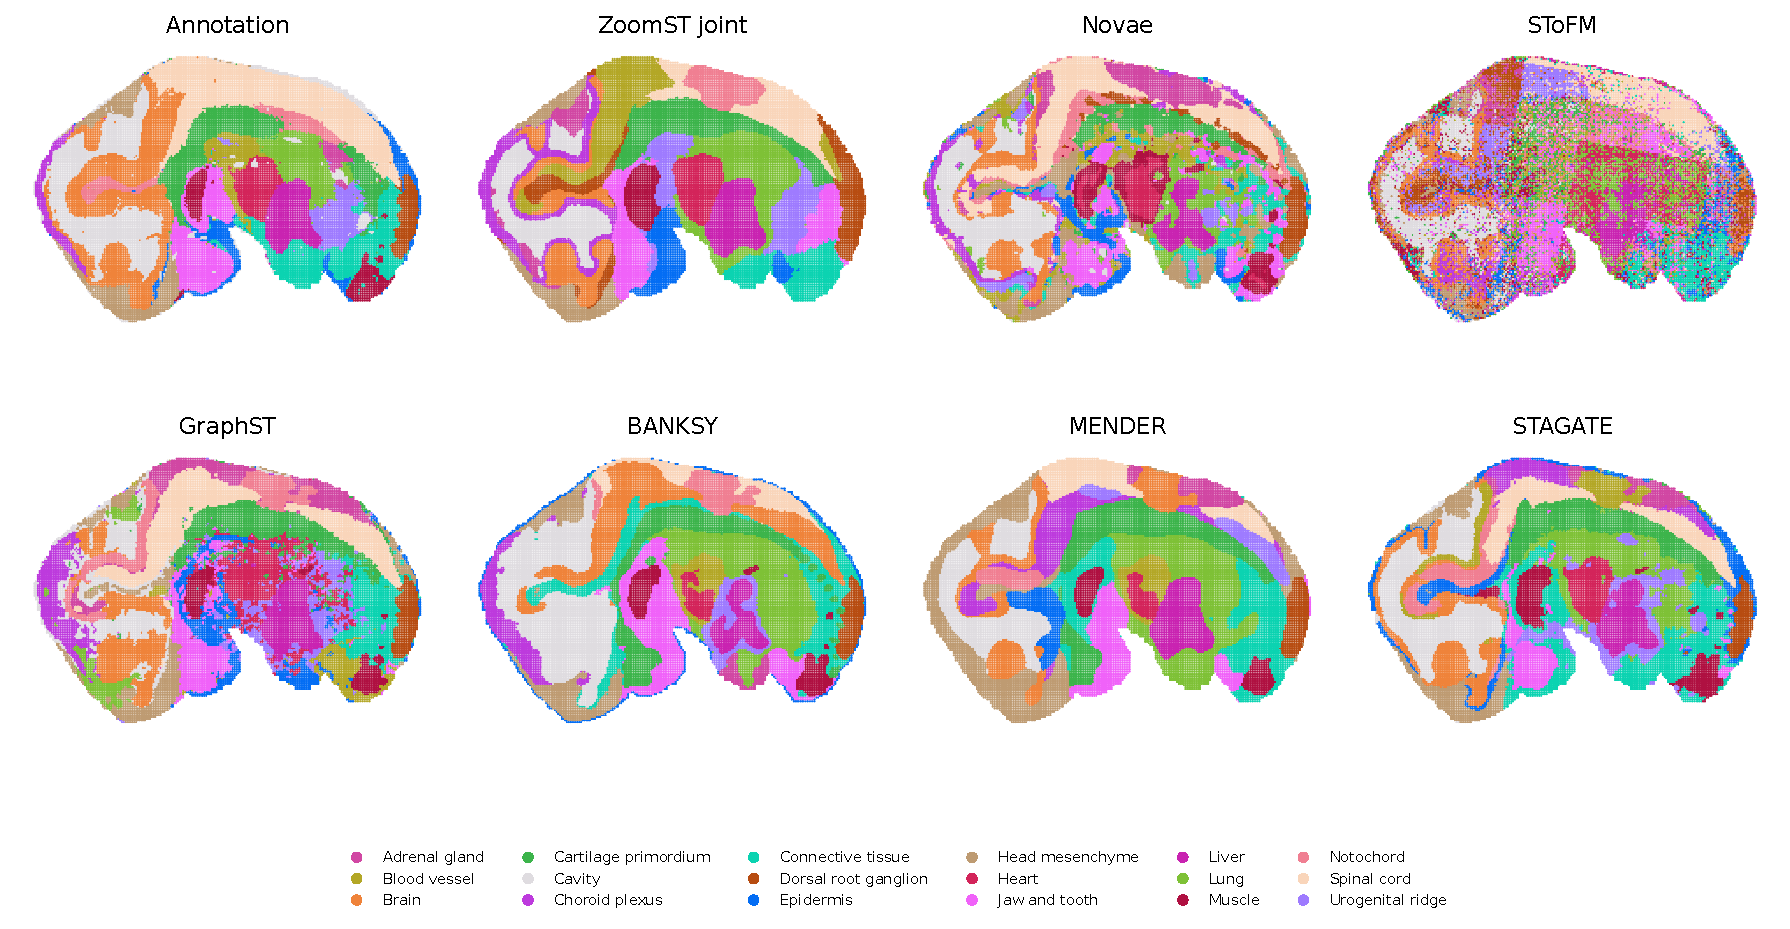
\includegraphics[width=\linewidth]{figures/e125_full_section.pdf}
\caption{\textbf{Example case: whole-section tissue mapping in E12.5 E2S1.} The annotation and seven-method predictions share all 23,640 positions and 18 primary classes. Maximum-overlap one-to-one matching assigns anatomical colors. The top row contains annotation and frozen pretrained features; the lower row contains target-fitted methods. Maps use no smoothing or label interpolation.}
\label{fig:dual-view-e125}
\end{figure}

\begin{figure}[!htbp]
\centering
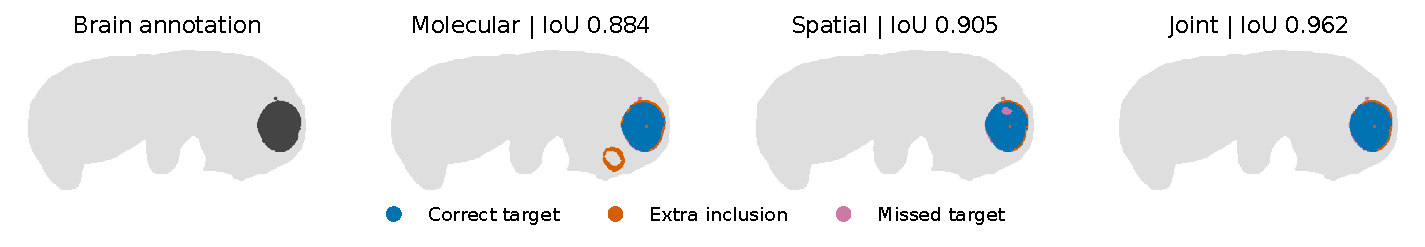
\includegraphics[width=\linewidth]{figures/brain_complementarity.pdf}
\caption{\textbf{Complementary molecular and spatial errors on a held-out section.} Annotation, molecular, spatial, and joint Brain assignments in E16.5 E2S13. Blue: correct assignments; orange: extra assignments; magenta: missed Brain.}
\label{fig:dual-view-brain}
\end{figure}

\begin{figure}[!htb]
\centering
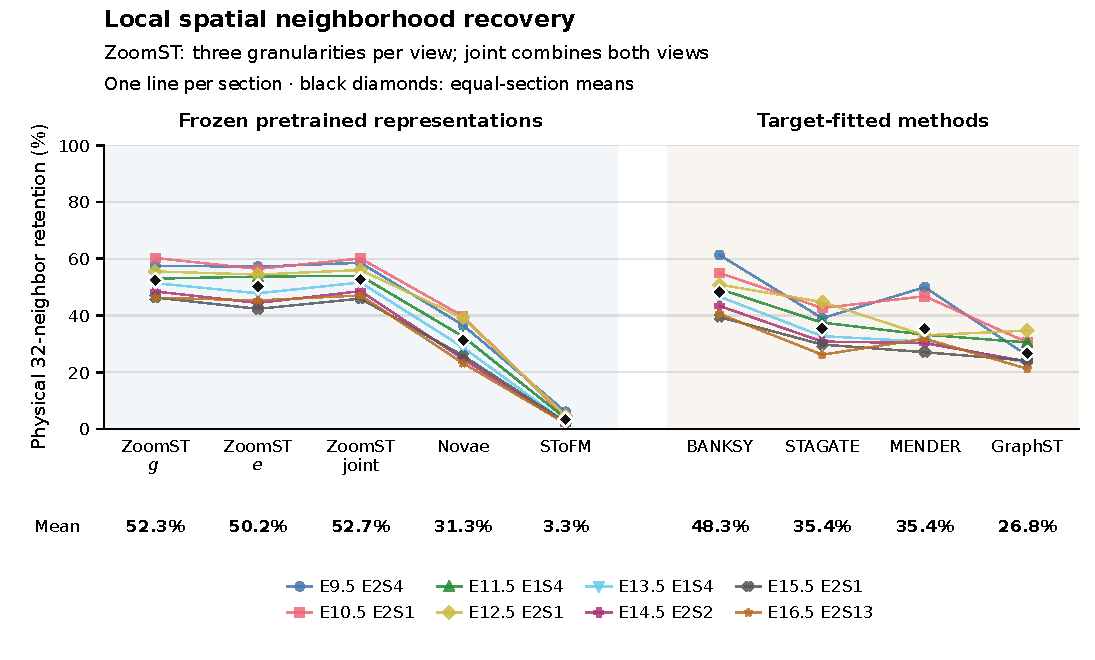
\includegraphics[width=\linewidth]{figures/spatial_retention_multiview.pdf}
\caption{\textbf{Local neighbor retention in the tissue-mapping representations.} Markers show physical 32-neighbor recovery over 2,048 fixed queries per section; all positions are candidates and self is excluded. Colored lines connect the same section within each method group, and black diamonds mark equal-section means. ZoomST $g$ and $e$ each concatenate granularities 8, 32, and 128; joint concatenates both views. All three use the same standardized PCA features as Table~\ref{tab:representation-summary}. Frozen pretrained representations and target-fitted spatial methods are grouped separately.}
\label{fig:dual-view-retention}
\end{figure}

\subsection{Developmental ordering and stage prediction within Brain}
\label{app:developmental-ordering}

MOSTA Brain is selected by coverage across all eight stages and the minimum available stage count. DPT uses the same 589 Brain observations from each held-out section, for 4,712 observations in total. HESTA Brain has sufficient coverage at CS17, CS18, CS19, CS20, and CS23; we fix 512 observations from each section, for 2,560 in total. Models share the same positions within each atlas. ZoomST and No Cross use the frozen models and Joint features defined in Appendix~\ref{app:dual-view}; the cross-method MOSTA comparison additionally uses Novae and SToFM's frozen embeddings and the shared-fit baselines below.

Table~\ref{tab:cross-granularity-development}b evaluates Joint separately at each context size $k\in\{8,32,128\}$. Within each atlas, all six model--scale combinations use the same balanced Brain cohort, 30 neighbors, and a fixed root. Each developmental stage is represented by one held-out section. Table~\ref{tab:joint-scale-comparison} additionally retains the MOSTA whole-section anatomical and physical-neighbor readouts alongside DPT.

\paragraph{Shared representations across sections.}
For the cross-method MOSTA comparison, GraphST and STAGATE each fit one encoder jointly across all eight target sections with shared gene selection and separate within-section spatial graphs. BANKSY uses a common 3,000-gene panel, and MENDER uses a common codebook of 32 unsupervised expression states. These fits use the complete target sections before extracting the balanced Brain observations. Other feature-construction and model-training settings follow Appendix~\ref{app:dual-view}.

\paragraph{Pseudotime.}
External baselines in both atlases share featurewise z-score standardization over the pooled Brain cohort, followed by PCA32 (STAGATE retains its native 30 dimensions). DPT~\citep{haghverdi2016dpt} uses Euclidean neighbor graphs and Scanpy's default distance definition with ten diffusion components.\footnote{\url{https://scanpy.readthedocs.io/en/stable/generated/scanpy.tl.dpt.html}} The default neighborhood size is 30. To address DPT computation failures, we expand the graph to 50 neighbors for STAGATE, BANKSY, and MENDER on MOSTA. Other DPT settings are shared. The MOSTA root is the E9.5 observation nearest the spatial centroid of the sampled E9.5 Brain domain. Sampling and numerical routines use seed 42. Root distances are normalized by the largest finite distance within each method; all selected MOSTA observations have finite pseudotime under the reported settings.

\paragraph{Pseudotime--stage agreement.}
For observation $i$, let $t_i$ denote pseudotime and $s_i$ its measured developmental stage. Spot-level Spearman correlation is $\operatorname{Spearman}(t_i,s_i)$ over all selected observations in an atlas, using unrounded pseudotimes and average ranks for ties. The observations span eight MOSTA stages or five HESTA stages. Figure~\ref{fig:developmental-ordering} reports both atlases; Table~\ref{tab:developmental-ordering} retains the combined-granularity MOSTA values.

For HESTA, the root is the first observation in the sorted sampled CS17 indices, fixed before evaluating the scores; its distances are normalized by the largest finite distance. ZoomST and No Cross have finite pseudotime for all selected Brain observations. Carnegie stage numbers specify the ordered target. PCA and graph construction pool the unlabeled Brain observations within each atlas; stage labels anchor the earliest-stage root and evaluate the resulting order.

\paragraph{HESTA cross-method comparison.}
The HESTA panel uses the same 2,560 Brain observations and CS17 root. Frozen external representations comprise Novae, SToFM, scGPT-spatial, the Cell, Neighborhood, and Spatial-cell outputs of TERRA, and CellWorld. They follow the standardization and DPT protocol above, with 30 neighbors for every method. CellWorld uses its frozen CP10K/log1p and per-section Seurat-HVG300 export. Its 512 CS18 observations are disconnected from the common root, so the figure marks its complete-stage readout as NA. The remaining methods cover all five stages. The existing independently fitted per-section DECIPHER embeddings are not pooled into a shared cross-stage coordinate system.

\begin{table}[!htbp]
\centering\scriptsize
\caption{\textbf{MOSTA Joint readouts by granularity.} AMI means follow Table~\ref{tab:cross-granularity-ami}a; SD is the sample SD across three downstream clustering runs. Neighbor retention is equal-section physical 32-neighbor recovery. Spot-level correlation uses the 4,712-observation Brain cohort. Bold marks the higher value in each pair, including ties.}
\label{tab:joint-scale-comparison}
\setlength{\tabcolsep}{2.2pt}
\renewcommand{\arraystretch}{1.18}
\begin{tabular}{l*{9}{c}}
\toprule
 & \multicolumn{3}{c}{AMI $\uparrow$} & \multicolumn{3}{c}{Neighbor retention (\%) $\uparrow$} & \multicolumn{3}{c}{Spot-level $\rho\uparrow$} \\
\cmidrule(lr){2-4}\cmidrule(lr){5-7}\cmidrule(lr){8-10}
Model & 8 & 32 & 128 & 8 & 32 & 128 & 8 & 32 & 128 \\
\midrule
ZoomST & \textbf{0.585 $\pm$ 0.006} & \textbf{0.571 $\pm$ 0.003} & 0.538 $\pm$ 0.002 & \textbf{35.1} & \textbf{52.7} & \textbf{62.5} & 0.868 & \textbf{0.822} & \textbf{0.354} \\
No Cross & 0.570 $\pm$ 0.001 & 0.562 $\pm$ 0.005 & \textbf{0.539 $\pm$ 0.0003} & 34.2 & 50.5 & 61.4 & \textbf{0.903} & 0.738 & -0.239 \\
\bottomrule
\end{tabular}

\end{table}

\begin{table}[!htbp]
\centering\small
\caption{\textbf{Spot-level pseudotime--stage Spearman correlation within Brain.} Correlation is computed over all 4,712 observations spanning eight MOSTA stages. Bold marks the highest value.}
\label{tab:developmental-ordering}
\setlength{\tabcolsep}{10pt}
\renewcommand{\arraystretch}{1.05}
\begin{tabular}{lc}
\toprule
Representation & \shortstack{Spot-level\\Spearman $\rho$} \\
\midrule
ZoomST joint & \textbf{0.816} \\
Novae & 0.714 \\
SToFM & 0.341 \\
ZoomST no cross & 0.651 \\
GraphST & 0.491 \\
STAGATE & 0.229 \\
BANKSY & -0.267 \\
MENDER & 0.458 \\
\bottomrule
\end{tabular}

\end{table}

\paragraph{Developmental-stage prediction.}
The linear probe uses the original Joint features without PCA. Each leave-one-section-out fold fits StandardScaler and a Ridge regressor only on Brain observations from the remaining sections. The intercept is unpenalized and the Ridge coefficient is $\alpha=n_{\mathrm{train}}\lambda$, with fixed $\lambda=0.1$. MOSTA training folds use 512 Brain observations per section and evaluate every Brain observation in the test section. HESTA uses the same fixed 512-observation-per-section cohort for training and testing across folds. Targets are embryonic days for MOSTA and Carnegie stages for HESTA. Encoder weights remain frozen throughout.

For section $s$ with $n_s$ evaluated observations, $\mathrm{MAE}_s=n_s^{-1}\sum_i|\hat{s}_i-s|$; reported MAE averages the included sections equally. Relative reduction is $(\overline{\mathrm{MAE}}_{\mathrm{No\ Cross}}-\overline{\mathrm{MAE}}_{\mathrm{ZoomST}})/\overline{\mathrm{MAE}}_{\mathrm{No\ Cross}}$.
\FloatBarrier


\section{Cross-granularity prediction}
\label{app:granularity-transfer}

\paragraph{Representation states.}
The final MOSTA model specified in Section~\ref{sec:experiments} supplies native 256-dimensional molecular states without standardization. Data use follows Table~\ref{tab:evaluation_protocol}.

\paragraph{Same-location state prediction.}
For every position in each section, define $m_i^T=d^{-1}\|T_{a\to b}(e_{i,a})-e_{i,b}\|_2^2$ and $m_i^0=d^{-1}\|e_{i,a}-e_{i,b}\|_2^2$. Figure~\ref{fig:granularity-transfer}A reports $\rho_{ab}=\sum_i m_i^T/\sum_i m_i^0$ for each section. The unchanged source is the no-transformation reference; the target is directly encoded from the actual broader neighborhood at the same location. Improved-position fractions use $n^{-1}\sum_i\mathbf 1[m_i^T<m_i^0]$. Scores are computed over all positions in each evaluated section. This evaluation differs from training, where all centers within each coarse support contribute sources.

\paragraph{Projected joint association.}
Each section supplies the same fixed 2,048 positions, partitioned into four disjoint batches of 512. For each batch, correct predicted pairings, unchanged-source controls, and 20 shuffled predictions are compared with directly encoded fine--coarse pairs. Each shuffle has no fixed points and permutes only predicted destinations, preserving their marginal distribution. The product kernel uses source and target bandwidths from the corresponding observed states, shared across controls, with the settings in Appendix~\ref{app:hyperparameters}.

We evaluate the checkpoint's training projection and eight fixed orthogonal projections with seeds 2026091501--2026091508. Figure~\ref{fig:granularity-transfer}B divides the mean correct-pair MMD by the mean shuffled MMD after averaging batches and the eight fresh projections within each section. Correct pairing improves on shuffling in all 864 batch--projection--direction conditions. Compared with the unchanged source on the training projection, transformation lowers joint discrepancy in 21 of 24 section--direction conditions. All three exceptions are in E12.5 E2S1; its projected joint discrepancy increases for each training direction. Table~\ref{tab:granularity-transfer-sections} reports every section and direction.

\begin{figure}[!htbp]
\centering
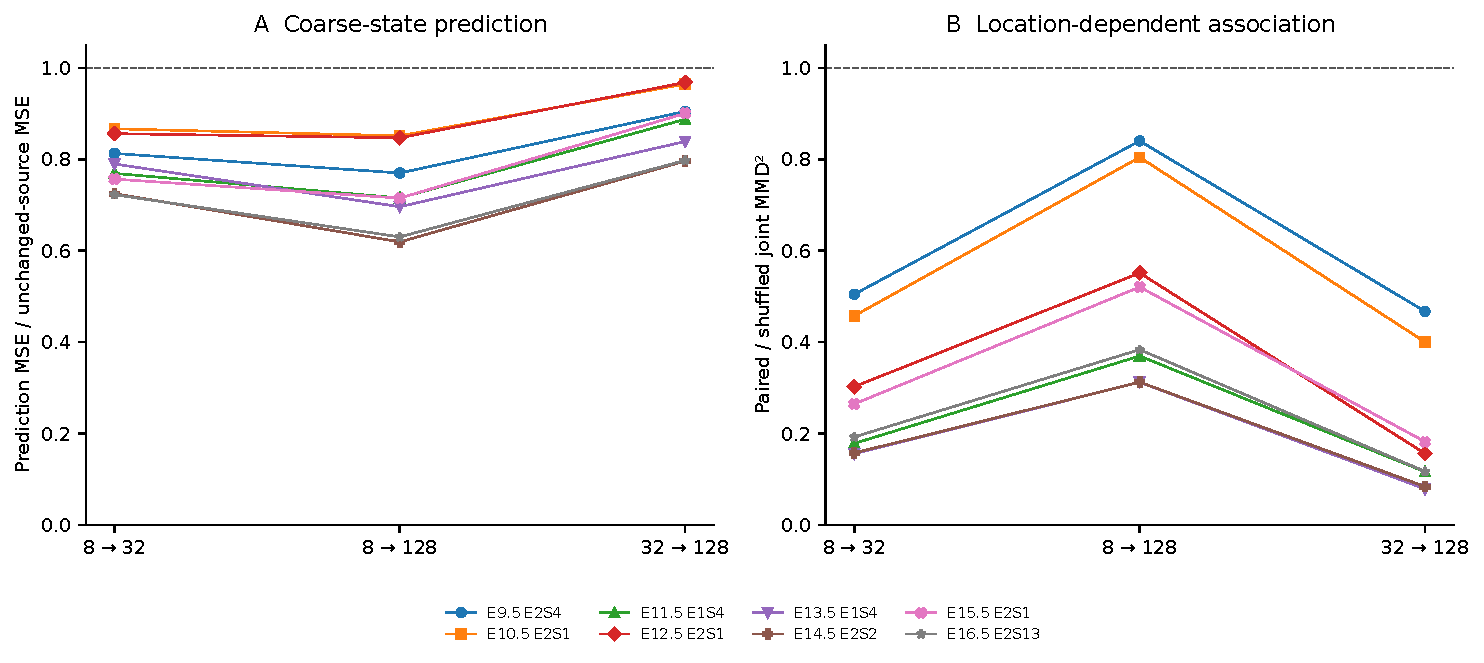
\includegraphics[width=\linewidth]{figures/granularity_transfer.pdf}
\caption{\textbf{Predictive relationships across held-out tissue sections.} \textbf{A}, Target-MSE ratio of transformed to untransformed fine states, using the same directly encoded coarse reference. \textbf{B}, Joint-MMD ratio of correct to shuffled predicted pairings, averaged over four batches and eight projections unused in training. Each line denotes one section; values below one favor the learned prediction or correct pairing.}
\label{fig:granularity-transfer}
\end{figure}

\begin{table}[!htbp]
\centering\small
\caption{\textbf{Coarse-state prediction on every held-out section.} MSE ratio compares transformed and unchanged sources against the same encoded coarse target. Improved is the percentage of positions with lower MSE. Paired/shuffled is the joint-MMD ratio averaged over batches and fresh projections.}
\label{tab:granularity-transfer-sections}
\begin{tabular}{lcccc}
\toprule
Section & Pair & MSE ratio & Improved (\%) & Paired/shuffled \\
\midrule
E9.5 E2S4 & 8$\to$32 & 0.813 & 98.0 & 0.505 \\
E9.5 E2S4 & 32$\to$128 & 0.905 & 84.3 & 0.467 \\
E9.5 E2S4 & 8$\to$128 & 0.770 & 98.3 & 0.840 \\
E10.5 E2S1 & 8$\to$32 & 0.867 & 88.7 & 0.458 \\
E10.5 E2S1 & 32$\to$128 & 0.965 & 58.7 & 0.400 \\
E10.5 E2S1 & 8$\to$128 & 0.851 & 88.7 & 0.804 \\
E11.5 E1S4 & 8$\to$32 & 0.769 & 97.9 & 0.178 \\
E11.5 E1S4 & 32$\to$128 & 0.888 & 82.3 & 0.116 \\
E11.5 E1S4 & 8$\to$128 & 0.715 & 98.2 & 0.370 \\
E12.5 E2S1 & 8$\to$32 & 0.856 & 88.9 & 0.302 \\
E12.5 E2S1 & 32$\to$128 & 0.968 & 53.7 & 0.156 \\
E12.5 E2S1 & 8$\to$128 & 0.847 & 84.1 & 0.551 \\
E13.5 E1S4 & 8$\to$32 & 0.790 & 97.4 & 0.156 \\
E13.5 E1S4 & 32$\to$128 & 0.839 & 89.0 & 0.079 \\
E13.5 E1S4 & 8$\to$128 & 0.696 & 98.5 & 0.312 \\
E14.5 E2S2 & 8$\to$32 & 0.725 & 98.6 & 0.157 \\
E14.5 E2S2 & 32$\to$128 & 0.796 & 91.9 & 0.084 \\
E14.5 E2S2 & 8$\to$128 & 0.619 & 99.5 & 0.312 \\
E15.5 E2S1 & 8$\to$32 & 0.757 & 93.9 & 0.265 \\
E15.5 E2S1 & 32$\to$128 & 0.900 & 59.2 & 0.182 \\
E15.5 E2S1 & 8$\to$128 & 0.715 & 91.7 & 0.521 \\
E16.5 E2S13 & 8$\to$32 & 0.722 & 97.9 & 0.192 \\
E16.5 E2S13 & 32$\to$128 & 0.798 & 91.4 & 0.117 \\
E16.5 E2S13 & 8$\to$128 & 0.630 & 98.3 & 0.383 \\
\bottomrule
\end{tabular}

\end{table}


\clearpage
\section{Unseen granularities and context response}
\label{app:scale-continuum}

\paragraph{Figure~\ref{fig:granularity-query-summary}: evaluation and aggregation.}
All three panels use eight sections excluded from pretraining, with the encoder and transformation frozen. In panels (a,b), target MSE compares unchanged source states and ZoomST predictions against the same directly encoded targets. Panel (a) averages the trained pairs $8\to32$, $8\to128$ and $32\to128$ within each section, using all section positions. Panel (b) averages the six unseen targets $12,16,24,48,64,96$ queried from $e_8$ at 1,024 fixed positions per section. Panel (c) selects the lowest and highest predicted-response quarters separately within each section and doubling interval ($8\to16$, $16\to32$, $32\to64$, $64\to128$), with 256 locations per quarter, then averages their directly encoded changes over the four intervals. Each box therefore contains eight section means. The highest-response quarter shows larger encoded changes than the lowest quarter in 31 of 32 section--interval conditions (Figure~\ref{fig:granularity-query-summary}c).

\subsection{Transition heads on a shared frozen encoder}
\label{app:transition-comparison}

\paragraph{Shared-encoder comparison.}
The neural ODE and granularity-conditioned residual MLP are trained at 8, 32 and 128 on a shared frozen encoder, then evaluated against the same directly encoded targets. Averaging MSE over six unseen granularities, the ODE reduces error on every held-out section, with a mean paired reduction of 10.86\% (Figure~\ref{fig:ode-transition-comparison}).

\begin{figure}[!htbp]
\centering
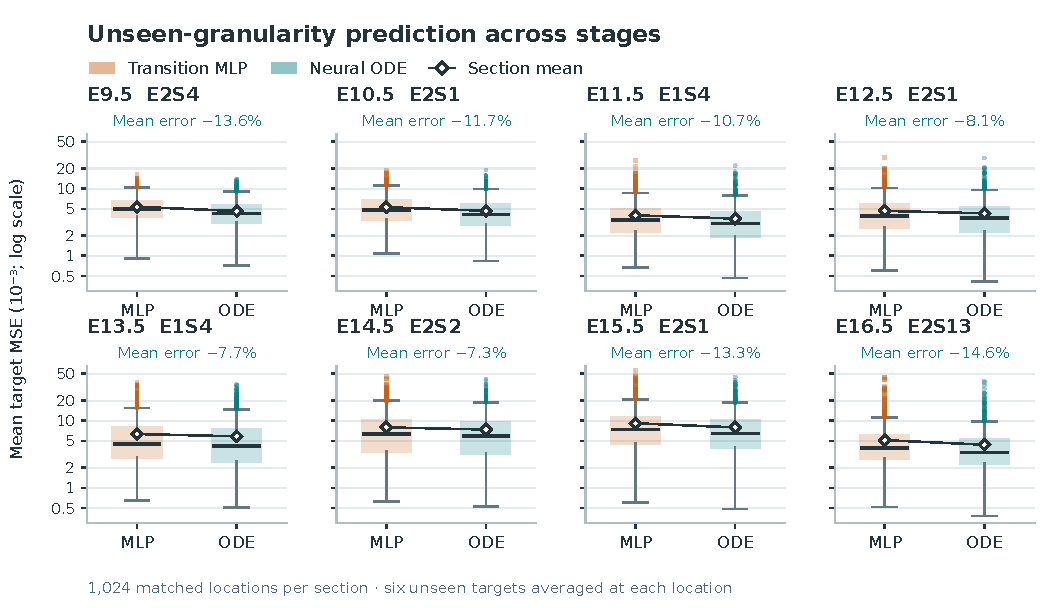
\includegraphics[width=\linewidth]{figures/ode_vs_transition_boxplots.pdf}
\caption{\textbf{Lower mean unseen-granularity error with neural ODE.} Each panel compares the granularity-conditioned residual MLP and ODE on one held-out section. Both heads use the same frozen encoder, fine-state inputs and directly encoded targets. Each box contains 1,024 location-level MSEs, each averaged equally over $k\in\{12,16,24,48,64,96\}$. Boxes show medians and interquartile ranges; whiskers extend to 1.5 interquartile ranges, with all outliers shown. Connected diamonds mark section means; percentages give their paired relative reductions. All panels share the same logarithmic axis.}
\label{fig:ode-transition-comparison}
\end{figure}

We compare the ODE with the granularity-conditioned residual MLP,
\[
T^{\mathrm{MLP}}_{a\to b}(z)=z+\mathrm{MLP}\!\left([\mathrm{LN}(z),h(a),h(b),u(b)-u(a)]\right).
\]
The MLP has dimensions $321\to128\to256$ with GELU activation and 32-dimensional scale embeddings; the ODE field has dimensions $257\to128\to256$. For a query between adjacent trained coordinates $u_j,u_{j+1}$, the MLP uses $h(k)=(1-w)h_j+wh_{j+1}$ with $w=(u(k)-u_j)/(u_{j+1}-u_j)$. The heads contain 74,848 and 66,560 trainable parameters, respectively.

Both heads are initialized afresh and trained on the same frozen encoder outputs from all 45 source sections for two epochs (7,224 updates; batch 1,024). AdamW uses learning rate $2\times10^{-4}$, 188 warmup steps and cosine decay to one tenth of the peak rate; gradient norms are clipped at five. Weight decay is 0.02 for weight matrices, 0.01 for scale embeddings and zero for normalization and bias terms. The ODE uses RK4 with maximum step 0.25 in $u$. Evaluation uses the same 1,024 positions per held-out section and the same directly encoded targets for both heads.

For section $s$, let $M_s^m$ be its MSE averaged equally over the six unseen targets for head $m$. The mean paired reduction is $100\,\mathrm{mean}_s(1-M_s^{\mathrm{ODE}}/M_s^{\mathrm{MLP}})=10.86\%$, ranging from 7.28\% to 14.56\% across sections. Table~\ref{tab:ode-transition-frozen} gives the section summaries underlying Figure~\ref{fig:ode-transition-comparison}. These are separately fitted transition heads on a common reference encoder.

\begin{table}[!htbp]
\centering\small
\caption{\textbf{Matched transition heads on a shared frozen encoder.} MSE is averaged over all six unseen targets and 1,024 locations per section. The mean reduction averages the eight paired section reductions.}
\label{tab:ode-transition-frozen}
\begin{tabular}{lccc}
\toprule
Section & MLP MSE ($\times10^{-3}$) & ODE MSE ($\times10^{-3}$) & Reduction (\%) \\
\midrule
E9.5 E2S4 & 5.381 & 4.650 & 13.57 \\
E10.5 E2S1 & 5.303 & 4.682 & 11.73 \\
E11.5 E1S4 & 4.014 & 3.585 & 10.69 \\
E12.5 E2S1 & 4.673 & 4.295 & 8.08 \\
E13.5 E1S4 & 6.342 & 5.853 & 7.71 \\
E14.5 E2S2 & 7.971 & 7.391 & 7.28 \\
E15.5 E2S1 & 9.174 & 7.957 & 13.26 \\
E16.5 E2S13 & 5.140 & 4.392 & 14.56 \\
Mean & 6.000 & 5.350 & 10.86 \\
\bottomrule
\end{tabular}

\end{table}

\subsection{Agreement with unseen neighborhood encodings}
\label{app:unseen-state-detail}

\paragraph{Frozen state prediction.}
The MOSTA encoder and ODE transition are frozen after joint training at 8,32,128. We use 1,024 fixed positions on each of the eight held-out sections and directly encode neighborhoods at $\mathcal K=\{8,12,16,24,32,48,64,96,128\}$. The molecular encoding procedure and neighborhood ordering remain unchanged. All predictions start from the same $e_{i,8}$; the encoded intermediate states are scoring references and do not enter these predictions.

Let $\widehat e_i(k)=T_{8\to k}(e_{i,8})$ and $\mathcal U=\mathcal K\setminus\{8,32,128\}$. For section $s$, target MSE averages $d^{-1}\|\widehat e_i(k)-e_i(k)\|^2$ over positions. The section's relative gain is one minus its MSE averaged over $k\in\mathcal U$ divided by the corresponding unchanged-$e_8$ MSE. Gains are then averaged over eight sections, yielding 21.96\%. Normalized RMSE divides RMSE by the target's root-mean-square variation around its section mean, so $R^2=1-\mathrm{NRMSE}^2$ within each section. Prediction improves over unchanged $e_8$ in all 48 section--target conditions. Figure~\ref{fig:granularity-query-summary}b plots absolute MSE averaged over the six targets within each section, giving eight paired section means.

\paragraph{Distance to a common directly encoded target.}
For the direct-distance comparison in Figure~\ref{fig:ode-unseen-distance-distributions}, define
\[
d_i^{\mathrm{start}}(k)=\frac{\|e_{i,8}-e_i(k)\|_2}{\sqrt d},\qquad
d_i^{\mathrm{pred}}(k)=\frac{\|\widehat e_i(k)-e_i(k)\|_2}{\sqrt d}.
\]
At each target, we average these per-position RMS distances within each section. Sections receive equal weight in the summary. Averaging $1-\overline d_s^{\mathrm{pred}}(k)/\overline d_s^{\mathrm{start}}(k)$ equally over the six unseen targets and eight sections gives a 10.38\% reduction, ranging from 3.04\% to 20.55\% across the 48 conditions. Every condition has a lower mean and median prediction distance. Within individual conditions, 81.15--99.71\% of positions are closer to the target. This RMS-distance statistic differs from the reduction in mean squared error reported above.

\begin{figure}[!htbp]
\centering
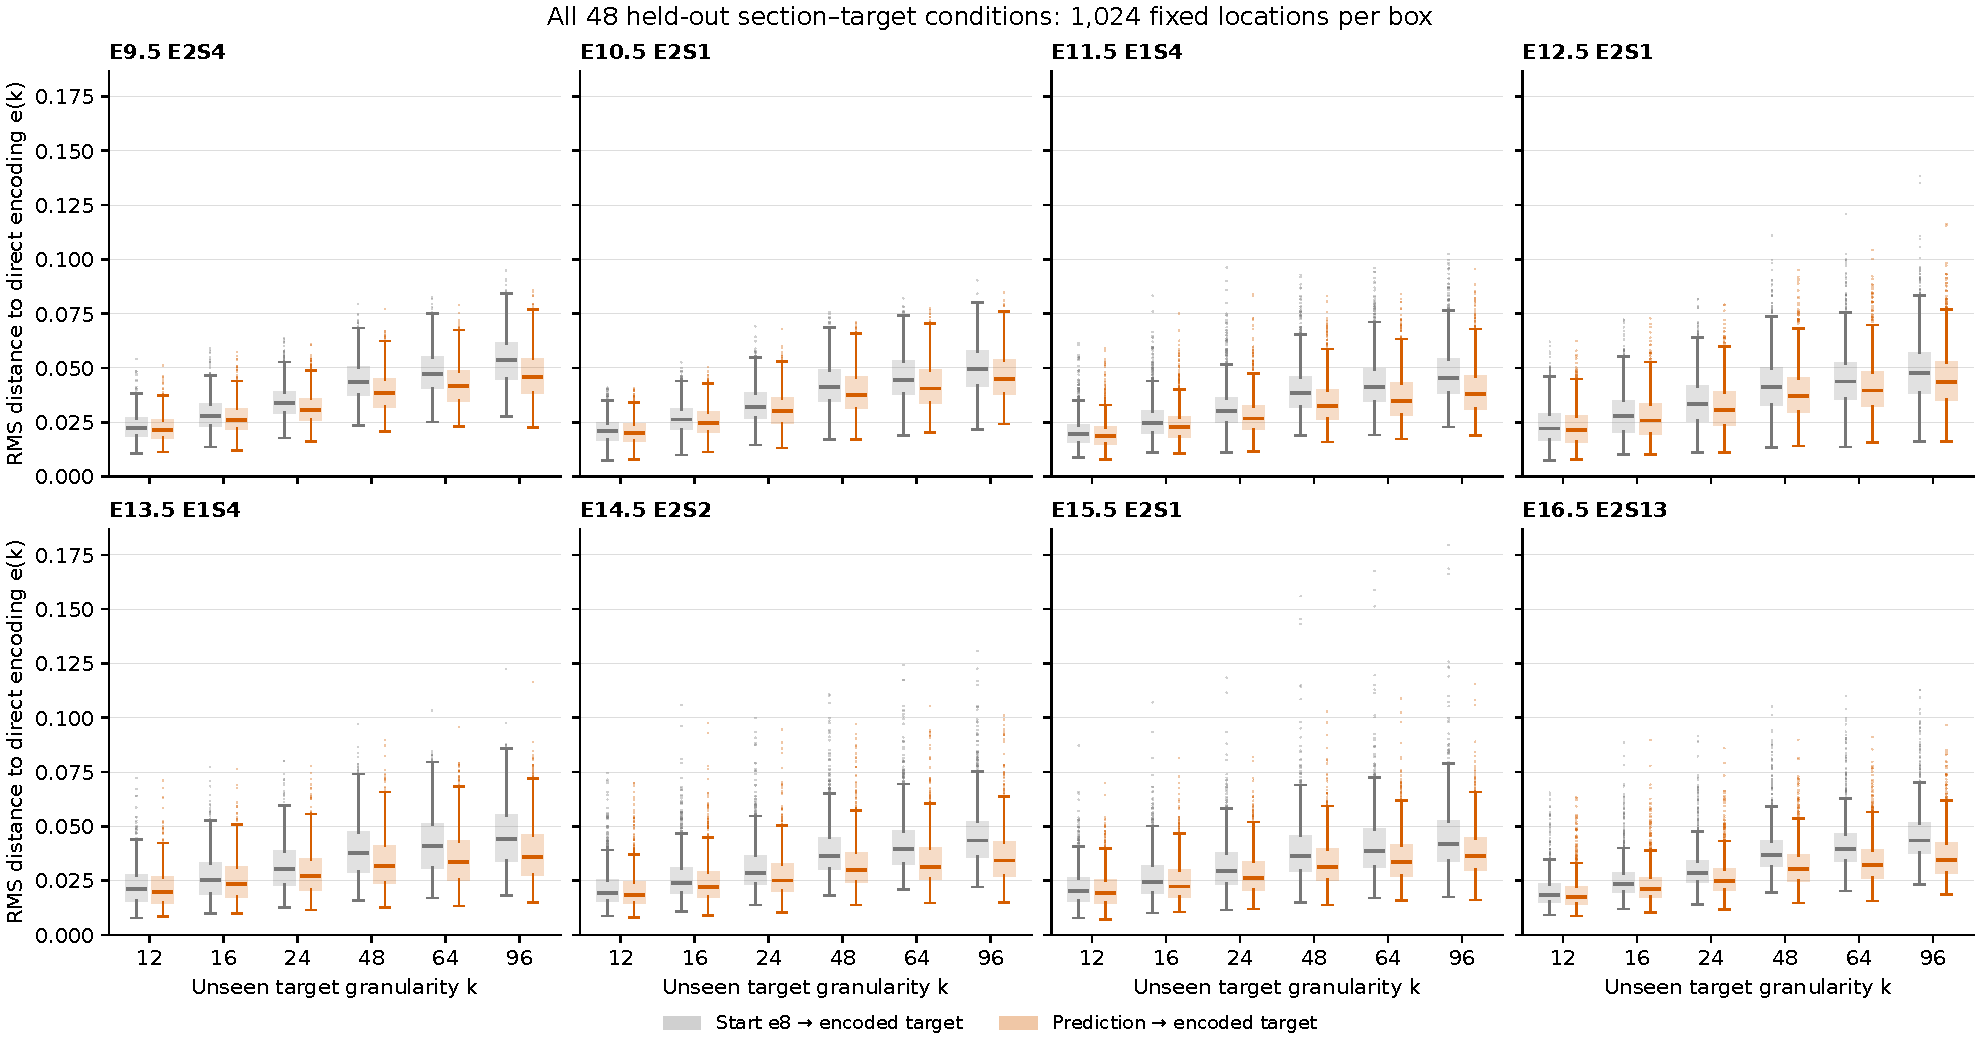
\includegraphics[width=\linewidth]{figures/unseen_state_distances_all_sections.pdf}
\caption{\textbf{Within-section distributions of distance to directly encoded unseen states.} The panels cover eight held-out sections and six unseen target granularities. Each pair compares distances from unchanged $e_8$ and from the prediction to the same target at the same 1,024 fixed positions. Boxes show medians and interquartile ranges, whiskers extend to 1.5 interquartile ranges, and outliers are retained. Position distributions describe each section; section means are the units in the main comparison.}
\label{fig:ode-unseen-distance-distributions}
\end{figure}

\paragraph{Shared-space visualization and full-state error.}
The E16.5 E1S1 analysis uses 1,024 fixed positions. We fit a center-only, full-SVD PCA on the directly encoded states at all nine granularities, then apply the same mean and components to predictions. All positions are shown with common axis limits. The first two PCs explain 20.25\% and 17.02\% of encoded-state variance. Table~\ref{tab:ode-case-pca} reports prediction accuracy in the full 256-dimensional space.

\begin{figure}[!htbp]
\centering
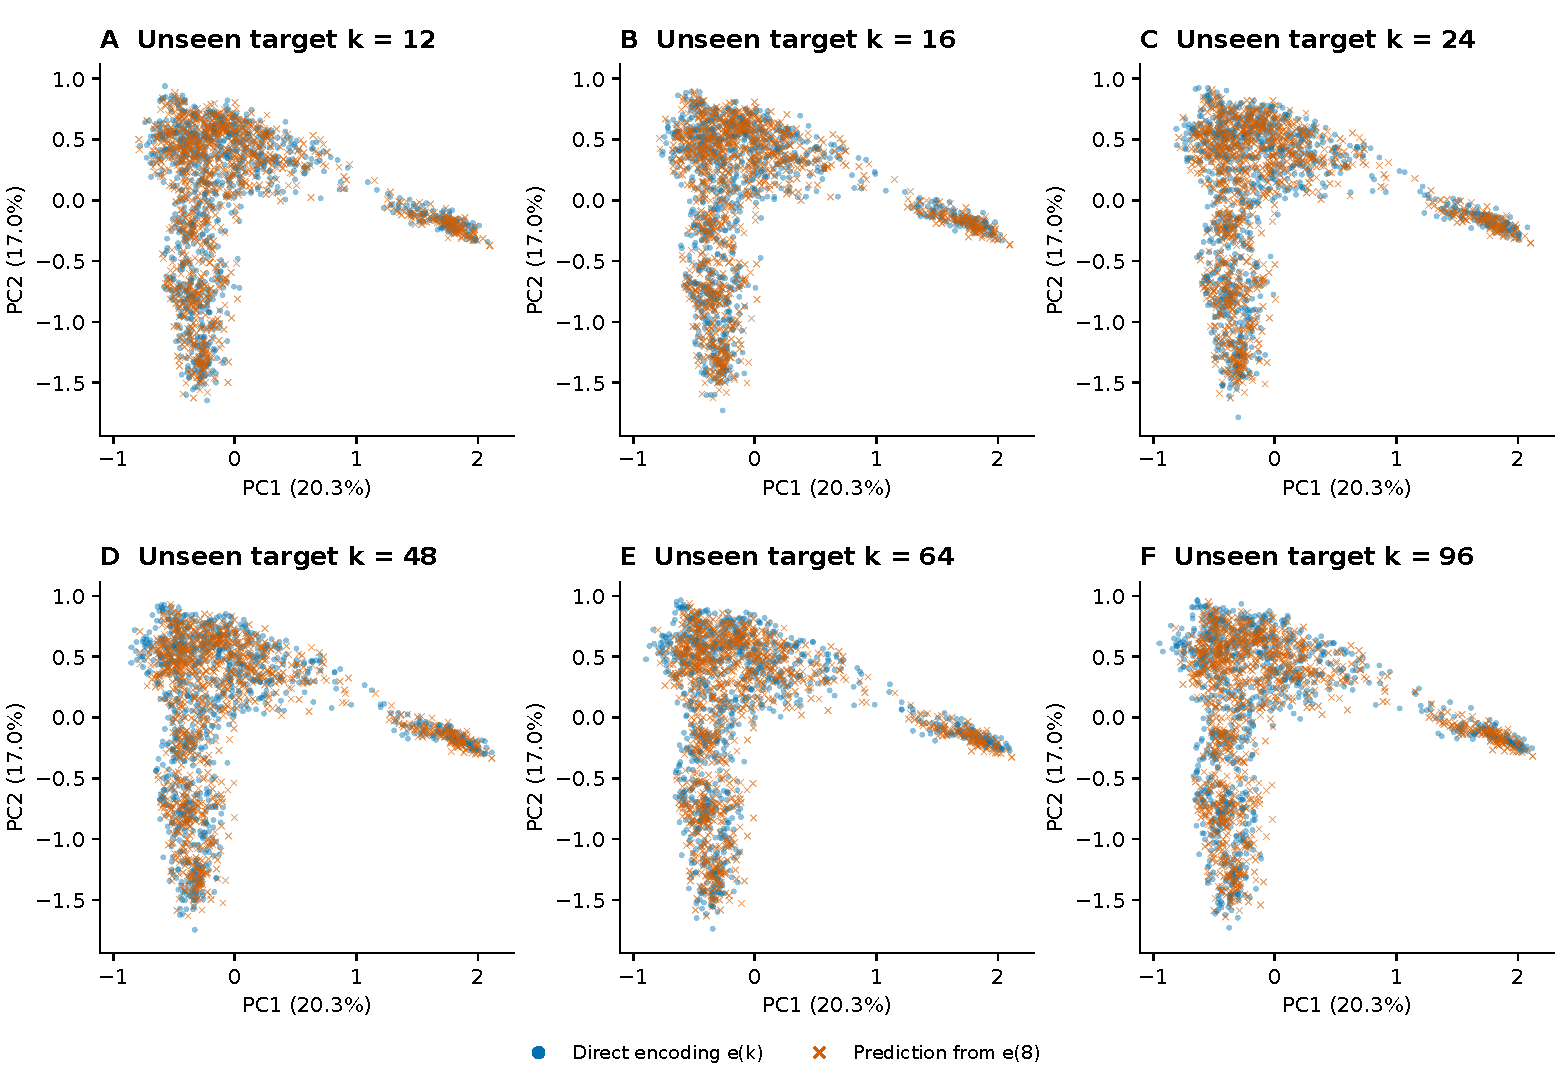
\includegraphics[width=\linewidth]{figures/case_all_unseen_pca_no_pair_lines.pdf}
\caption{\textbf{All six unseen target states in the E16.5 E1S1 case.} Every panel uses the same PCA basis and the same 1,024 positions. Metrics are computed in 256 dimensions. Targets and predictions are paired at each location.}
\label{fig:ode-case-all-pca}
\end{figure}
\begin{table}[!htbp]
\centering\small
\caption{\textbf{Full-dimensional accuracy underlying the case PCA.} MSE ratio compares prediction with unchanged $e_8$ against directly encoded targets; NRMSE and $R^2$ use the same full-dimensional targets.}
\label{tab:ode-case-pca}
\begin{tabular}{lccc}
\toprule
Target $k$ & MSE ratio & NRMSE & $R^2$ \\
\midrule
12 & 0.884 & 0.206 & 0.958 \\
16 & 0.810 & 0.243 & 0.941 \\
24 & 0.739 & 0.280 & 0.922 \\
48 & 0.664 & 0.333 & 0.889 \\
64 & 0.643 & 0.352 & 0.876 \\
96 & 0.621 & 0.377 & 0.858 \\
\bottomrule
\end{tabular}

\end{table}

\FloatBarrier
\subsection{Context-response evaluation across observation ranges}
\label{app:response-meaning}

\paragraph{Matched response definitions and sampling.}
For $\widehat e_i(k)=T_{8\to k}(e_{i,8})$, Figure~\ref{fig:granularity-query-summary}c, Figure~\ref{fig:ode-context}a and the grouping in Figure~\ref{fig:facial-nerve-composition} use
\[
D_i^{\mathrm{pred}}(a,b)=
\frac{\|\widehat e_i(b)-\widehat e_i(a)\|_2}{\sqrt d\,\log_2(b/a)},\qquad
D_i^{\mathrm{enc}}(a,b)=
\frac{\|e_i(b)-e_i(a)\|_2}{\sqrt d\,\log_2(b/a)}.
\]
Both operands in the predicted displacement belong to queries from the same fixed $e_8$. Encoded states are evaluation references, and all displayed doubling intervals have log width one.

Held-out comparisons use 1,024 fixed locations per section. Anatomical cases use the training sections identified in Table~\ref{tab:evaluation_protocol}, with up to 128 locations per annotation selected by a fixed hash of observation identity; smaller domains retain every location.

\paragraph{Held-out location ordering.}
For each held-out section and each doubling interval, we sort the 1,024 locations by predicted response and split them into four equal groups; ties preserve sample order. We compare the directly encoded changes in the lowest and highest quarters. Figure~\ref{fig:granularity-query-summary}c averages these group means over the four intervals within each section, giving eight paired section means.

\paragraph{Actual neighborhood composition.}
Let $q_{ic}(k)$ be the proportion of annotation $c$ among the $k-1$ neighbors after excluding the focal center. For the same interval as the response,
\[
C_i(a,b)=\tfrac12\sum_c|q_{ic}(b)-q_{ic}(a)|.
\]
Support ordering is identical to the model input, and unknown-label mass is retained. The Facial nerve composition bars (Figure~\ref{fig:facial-nerve-composition}) follow the same 16 locations in each extreme predicted-response quarter. Their mean encoded changes are 0.0191 and 0.0343 in the low and high groups, respectively (ratio 1.799). Corresponding mean TV values are 0.134 and 0.284. Composition TV quantifies the change in annotated tissue proportions.

\begin{figure}[!htbp]
\centering
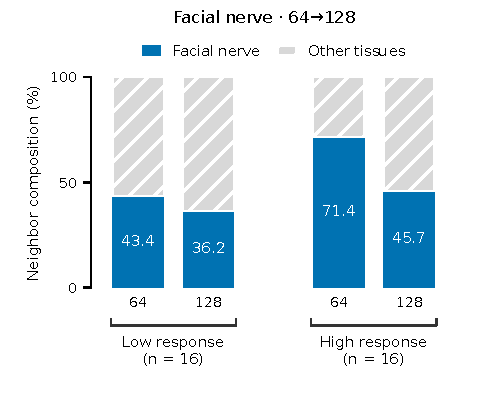
\includegraphics[width=0.58\linewidth]{figures/facial_nerve_composition.pdf}
\caption{\textbf{Neighborhood composition in low- and high-response Facial nerve locations.} The groups are the lowest and highest predicted-response quarters among all 64 Facial nerve locations in the E14.5 E1S1 training section, using the $64\to128$ response in Figure~\ref{fig:ode-context}a. Each pair of bars follows the same 16 locations at both granularities. Blue shows the mean Facial nerve fraction; gray shows all other labels. Predictions start from fixed $e_8$.}
\label{fig:facial-nerve-composition}
\end{figure}

\paragraph{Within-Brain changes under a constant annotation.}
Among sampled Brain locations whose neighborhoods remain entirely Brain-labeled at both $r=8$ and $r=16$, predicted responses correlate with directly encoded changes (Spearman $\rho=0.645$), showing molecular-context variation within a constant anatomical annotation.

\paragraph{Whole-section spatial overview.}
Figure~\ref{fig:ode-context}b averages the instantaneous response $s_i(2^t)=\|f_\theta(z_i((t-3)/4),(t-3)/4)\|_2/(4\sqrt d)$ over 64 equally spaced midpoints in $t=\log_2 k\in[3,7]$. This path average differs from the finite response used in panel (a) and to define the groups in Figure~\ref{fig:facial-nerve-composition}. Colors use an empirical percentile reference pooled over the full-range mean and the four doubling-range means, with all 121,767 locations included. Panel (c) shows observed composition TV from 8 to 128. The maps show spatial distributions without smoothing; their whole-section Spearman correlation is 0.174. Both maps are rotated together by $180^\circ$ relative to the source coordinates for display, preserving distances and the common orientation. Spatial scale bars use the nominal $25\,\mu$m pitch of the bin50 matrices~\citep{chen2022mosta}; response remains normalized by $\log_2 k$.


\clearpage
\section{Objective ablation on MOSTA}
\label{app:objective-ablation}

We compare No Cross, CS, and ZoomST using a common initialization, the same training data and training budget, and identical training settings apart from the loss terms. No Cross uses within-granularity learning; CS adds coarse-support supervision; ZoomST further adds JointMMD. Evaluation uses frozen encoders and the held-out MOSTA split from Section~\ref{sec:developmental-information}, with identical evaluation observations and readout settings across the three models. All readouts use Joint representations at granularities 8, 32, and 128.

Table~\ref{tab:mosta-objective-ablation} follows the anatomical clustering, Brain developmental ordering, and stage-prediction protocols in Appendix~\ref{app:dual-view}--\ref{app:developmental-ordering}.

Adding JointMMD to CS reduces stage-prediction MAE and increases spot-level DPT correlation at all three granularities, with the largest gains at granularity 128. AMI increases at granularities 8 and 32 and remains similar at granularity 128.

\begin{table}[!htbp]
\centering
\caption{\textbf{Controlled objective ablation on MOSTA.} Joint AMI, Brain spot-level DPT--stage Spearman correlation, and Brain stage-prediction MAE. AMI averages the eight held-out sections equally; $\pm$ denotes SD over downstream clustering runs. DPT and stage MAE use the protocols and aggregation of Table~\ref{tab:cross-granularity-development}b. Bold marks the best unrounded mean in each column.}
\label{tab:mosta-objective-ablation}
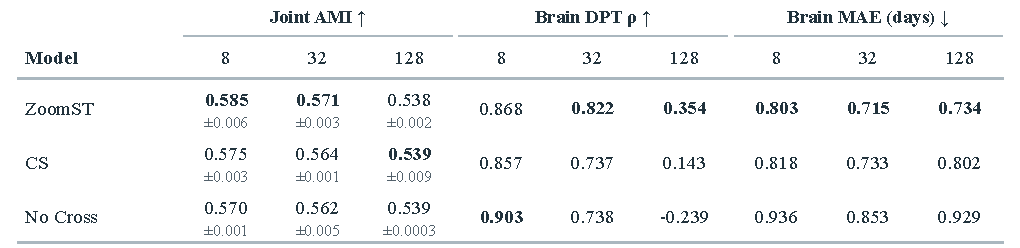
\includegraphics[width=\linewidth]{figures/mosta_objective_ablation.pdf}
\end{table}
\FloatBarrier



\end{document}
